\subsection{正项级数的收敛判别法}

在本节中，我们把（滥用语言的说法）这样的实项级数 \((u_{n})\) ：其项 \(u_{n} \geqslant 0\) 从 \(n\) 的某个特定值起成立，理解为正项级数。我们关于这类级数所说的一切，通过改变符号，立即可以推广到各项都 \(\leqslant 0\) （从 \(n\) 的某个特定值起）的级数。我们已经看到 (II, p.~64, 例 3)，对点的每个序列 \((\mathbf{u}_n)_{n\geqslant 1}\) （取值于赋范空间 \(E\) ），可以关联一个阶梯函数 \(\mathbf{u}\) ，它定义在 \([1, +\infty[\) 上，由条件 \(\mathbf{u}(x) = \mathbf{u}_n\) （对 \(n\leqslant x < n + 1\) ）确定：这时级数 \((\mathbf{u}_n)\) 收敛当且仅当积分 \(\int_1^{+\infty}\mathbf{u}(t)dt\) 收敛。

设 \((u_{n})\) 与 \((v_{n})\) 是两个正项级数，u 与 v 是相应的阶梯函数：关系 \(u_{n} \leqslant v_{n}\) （对 \(n \geqslant n_{0}\) ）等价于 \(u(x) \leqslant v(x)\) （对 \(x \geqslant n_{0}\) ）。于是关系 \(u_{n} \preccurlyeq v_{n}, u_{n} \prec v_{n}, u_{n} \sim v_{n}\) 中的每一个分别等价于 \(u(x) \preccurlyeq v(x), u(x) \prec v(x)\) 与 \(u(x) \sim v(x)\) ；这一注记使我们能把命题 1 (V, p.~228) 与命题 6 (V, p.~230) 表述如下：

命题 1. 设 \((u_{n})\) 与 \((v_{n})\) 是两个正项级数。若 \(u_{n} \preccurlyeq v_{n}\) 且级数 \((v_{n})\) 收敛，则 \((u_{n})\) 收敛；若 \(u_{n} \succcurlyeq v_{n}\) 且 \(\sum_{n=1}^{\infty} v_{n} = +\infty\) ，则 \(\sum_{n=1}^{\infty} u_{n} = +\infty\) 。

命题 2. 设 \((u_{n})\) 与 \((v_{n})\) 是两个正项级数：

\(1^{\circ}\) 若级数 \((v_{n})\) 收敛，则关系 \(u_{n} \ll v_{n}\) （相应地， \(u_{n} \sim v_{n}\) ）蕴含 \(\sum_{p=n}^{\infty} u_{p} \ll \sum_{p=n}^{\infty} v_{p}\) （相应地， \(\sum_{p=n}^{\infty} u_{p} \sim \sum_{p=n}^{\infty} v_{p}\) ）。

\(2^{\circ}\) 若 \(\sum_{n=1}^{\infty} v_n = +\infty\) ，则关系 \(u_n \ll v_n\) （相应地， \(u_n \sim v_n\) ）蕴含 \(\sum_{p=1}^{n} u_p \ll \sum_{p=1}^{n} v_p\) （相应地， \(\sum_{p=1}^{n} u_p \sim \sum_{p=1}^{n} v_p\) ）。

在命题 1 中取比较级数 \((v_{n})\) 为通项形如 \(v_{n} = f(n)\) 的级数（其中 \(f\) 是一个 \(\geqslant 0\) 的函数，对每个实数 \(x > x_0\) 有定义且在区间 \([x_0, +\infty[\) 上递减），便得到方便的收敛判别法；事实上：

命题 3（柯西–麦克劳林判别法）. 若 \(f\) 是一个 \(\geqslant 0\) 且在 \([x_0, +\infty[\) 上递减的函数，则以 \(v_n = f(n)\) 为通项的级数收敛当且仅当积分 \(\int_{x_0}^{+\infty} f(t) dt\) 收敛。

为证明这一点，只需注意：若 v 是与级数 \((v_{n})\) 相关联的阶梯函数，则由于 f 递减， \(v(x+1) \leqslant f(x) \leqslant v(x)\) 对每个 \(x \geqslant x_{0}\) 成立；于是该命题是比较原理 (II, p.~66, prop. 3) 的推论。

由于出现在积分的对数收敛判别法 (V, p.~229, prop. 2、3 与 4) 中的函数在某个区间 \([x_{0}, +\infty[\) 上递减，应用 V, p.~237 的命题 1 与命题 3，就得到下列判别法：

命题 4（“0 阶对数判别法”）. 设 \((u_{n})\) 是正项级数；若 \(u_{n} \preccurlyeq n^{\mu}\) 对某个 \(\mu < -1\) 成立，则级数 \((u_{n})\) 收敛；若 \(u_{n} \succcurlyeq n^{\mu}\) 对某个 \(\mu \geqslant -1\) 成立，则级数 \((u_{n})\) 的和为无穷。

命题 5（“p 阶对数判别法”）. 设 \((u_{n})\) 是正项级数。若 \(u_{n} \preccurlyeq \frac{1}{nl_{1}(n)l_{2}(n)\ldots l_{p-1}(n)(l_{p}(n))^{\mu}}\) 对某个 \(\mu > 1\) 成立，则级数 \((u_{n})\) 收敛；若 \(u_{n} \succcurlyeq \frac{1}{nl_{1}(n)l_{2}(n)\ldots l_{p-1}(n)(l_{p}(n))^{\mu}}\) 对某个 \(\mu \leqslant 1\) 成立，则级数 \((u_{n})\) 的和为无穷。

若 \(0 \leqslant q < 1\) ，则 \(q^n \preccurlyeq n^{-\mu}\) 对任何 \(\mu > 0\) 成立；再应用 0 阶对数判别法便证明了几何级数 \(\sum_{n=0}^{\infty} q^n\) 对 \(|q| < 1\) 收敛 (Gen.~Top., IV, p.~364)。若在命题 1 中取 \(v_n = q^n\) ，就得到一个可以写成如下形式的判别法（“柯西判别法”）：设 \((u_n)\) 是正项级数；若 \(\limsup_{n \to \infty} (u_n)^{1/n} < 1\) ，则级数 \((u_n)\) 收敛；若 \(\limsup_{n \to \infty} (u_n)^{1/n} > 1\) ，则级数 \((u_n)\) 的和为无穷。事实上，若 \(\limsup_{n \to \infty} (u_n)^{1/n} = a < 1\) ，则 \(u_n \preccurlyeq q^n\) 对每个 \(q\) （使 \(a < q < 1\) ）成立。反之，若 \(\limsup_{n \to \infty} (u_n)^{1/n} = a > 1\) ，则 \(u_n \geqslant q^n > 1\) 对无穷多个 \(n\) 的值成立（对任何 \(q\) ，满足 \(1 < q < a\) ）；由于 \(u_n\) 不趋于 0，有 \(\sum_{n=1}^{\infty} u_n = +\infty\) 。

这个判别法在整级数理论（我们将在以后研究它）中非常有用；但即便如此，它仍不能判定级数 \((1/n^{\alpha})\) 的收敛性，换句话说，它的应用范围比对数判别法狭窄得多。

\subsection{级数部分和的渐近展开}

对实变量 \(x\) （趋于 \(+\infty\) ），设 \(\mathcal{E}\) 是一个比较尺度，由这样的函数组成：其中每个函数都在整个区间 \([x_0, +\infty[\) （随函数而定）上有定义，且在该区间上 \(\geqslant 0\) 。设 \((\mathbf{u}_n)\) 是各项都属于完备赋范空间 \(E\) 的级数，使得 \(\mathbf{u}_n\) 有精确到 \(g_\alpha\) 的渐近展开，它相对于尺度 \(\mathcal{E}'\) （由 \(\mathbf{N}\) 上的、来自 \(\mathcal{E}\) 中函数的限制组成）：

\[
\mathbf {u} _ {n} = \sum_ {\lambda \leqslant \alpha} \mathbf {a} _ {\lambda} g _ {\lambda} (n) + \mathbf {r} _ {\alpha} (n).
\]

假设每个部分和 \(\sum_{m=1}^{n} g(m)\) （其中 \(g \in \mathcal{E}\) ）都有关于 \(\mathcal{E}'\) 的渐近展开。于是可以得到 \(\mathbf{s}_n = \sum_{m=1}^{n} \mathbf{u}_m\) 关于 \(\mathcal{E}'\) 的渐近展开；我们仍然区分两种情形：

\(1^{\circ}\sum_{n = 1}^{\infty}g_{\alpha}(n) = +\infty .\) 这时 (V,p.237,prop.2) 有 \(\sum_{m = 1}^{n}\mathbf{r}_{\alpha}(m)\ll \sum_{m = 1}^{n}g_{\alpha}(m);\)

根据假设，可以得到

\[
\sum_ {\lambda \leqslant \alpha} \mathbf {a} _ {\lambda} \left(\sum_ {m = 1} ^ {n} g (m)\right)
\]

(V, p.~222) 到某个精确度 \(g_{\sigma}\) 的渐近展开；若 \(cg_{\sigma}(n)\) 是 \(\sum_{m=1}^{n} g_{\alpha}(m)\) 的主部，则将有 \(\mathbf{s}_n\) 的精确到 \(g_{\min(\rho, \sigma)}\) 的渐近展开。

\(2^{\circ}\sum_{n = 1}^{\infty}g_{\alpha}(n)\) 收敛；这时设 \(\beta\) 是指标 \(\lambda \leqslant \alpha\) 中最小的一个，它使 \(\mathbf{a}_{\lambda}\neq 0\) 且使 \(\sum_{n = 1}^{\infty}g_{\lambda}(n)\) 收敛；则级数

\[
\mathbf {C} = \sum_ {n = 1} ^ {\infty} \left(\mathbf {u} _ {n} - \sum_ {\lambda <   \beta} \mathbf {a} _ {\lambda} g _ {\lambda} (n)\right)
\]

绝对收敛，并且可以写

\[
\mathbf {s} _ {n} = \sum_ {\lambda <   \beta} \mathbf {a} _ {\lambda} \left(\sum_ {m = 1} ^ {n} g _ {\lambda} (m)\right) + \mathbf {C} - \sum_ {\beta \leqslant \lambda \leqslant \alpha} \mathbf {a} _ {\lambda} \left(\sum_ {m = n + 1} ^ {\infty} g _ {\lambda} (m)\right) - \sum_ {m = n + 1} ^ {\infty} \mathbf {r} _ {\alpha} (m).
\]

此外，有 \(\sum_{m=n+1}^{\infty}\mathbf{r}_{\alpha}(m)\ll\sum_{m=n+1}^{\infty}g_{\alpha}(m)\) ；若 \(cg_{\sigma}(n)\) 是 \(\sum_{m=n+1}^{\infty}g_{\alpha}(m)\) 的主部，且若已有

\[
\sum_ {\lambda <   \beta} \mathbf {a} _ {\lambda} \left(\sum_ {m = 1} ^ {n} g _ {\lambda} (m)\right) + \mathbf {C} - \sum_ {\beta \leqslant \lambda \leqslant \alpha} \mathbf {a} _ {\lambda} \left(\sum_ {m = n + 1} ^ {\infty} g _ {\lambda} (m)\right)
\]

到精确度 \(g_{\rho}\) 的渐近展开，便由此得到 \(s_{n}\) 的精确到 \(g_{\min(\rho,\sigma)}\) 的渐近展开。于是问题归结为级数 \((g(n))\) （其中 \(g \in E\) ）的特殊情形。我们将看到，在某些条件之下，如何能直接得到 \(s_{n} = \sum_{m=1}^{n} g(m)\) 的主部（当 \(\sum_{n=1}^{\infty} g(n) = +\infty\) 时）或 \(r_{n} = \sum_{m=n+1}^{\infty} g(m)\) 的主部（当 \(\sum_{n=1}^{n} g(n) < +\infty\) 时）。

命题 6. 设 \(g\) 是一个实函数， \(>0\) 且单调，定义在区间 \([x_0, +\infty[\) 上（其中 \(x_0 \leqslant 1\) ），且使 \(\log g\) 与 \(x\) 1 阶可比较。

\(1^{\circ}\) 若 \(g\) 相对于 \(e^{x}\) 是无穷阶的，则有

\[
s _ {n} = \sum_ {m = 1} ^ {n} g (m) \sim g (n) \quad i f \quad \sum_ {n = 1} ^ {\infty} g (n) = + \infty ;\tag{1}
\]

\[
r _ {n} = \sum_ {m = n + 1} ^ {\infty} g (m) \sim g (n + 1) \quad i f \quad \sum_ {n = 1} ^ {\infty} g (n) <   + \infty .\tag{2}
\]

\(2^{\circ}\) 若 \(g\) 有有限阶 \(\mu\) （相对于 \(e^{x}\) ），则有

\[
s _ {n} = \sum_ {m = 1} ^ {n} g (m) \sim \frac {\mu}{1 - e ^ {- \mu}} \int_ {x _ {0}} ^ {n} g (t) d t \quad i f \quad \sum_ {n = 1} ^ {\infty} g (n) = + \infty ;\tag{3}
\]

\[
r _ {n} = \sum_ {m = n + 1} ^ {\infty} g (m) \sim \frac {\mu}{1 - e ^ {- \mu}} \int_ {n} ^ {\infty} g (t) d t \quad i f \quad \sum_ {n = 1} ^ {\infty} g (n) <   + \infty\tag{4}
\]

（数 \(\frac{\mu}{1 - e^{-\mu}}\) 在 (3) 与 (4) 中当 \(\mu = 0\) 时应换成 1）。

\(1^{\circ}\) 若 \(g\) 的阶为 \(+\infty\) （相对于 \(e^{x}\) ），则有 \(\log g \gg x\) ，从而按假设有 \(g' / g \gg 1\) ，即 \(g' \gg g\) ；因此 \(g\) 递增并趋于 \(+\infty\) （随 \(x\) ），从而 \(\sum_{n=1}^{\infty} g(n) = +\infty\) 。若 \(u\) 是与级数 \((g(n))\) 相关联的阶梯函数 (V, p.~237)，则 \(u(x) \leqslant g(x)\) 从 \(x\) 的某个值起成立，故 \(u \preccurlyeq g\) ，因而

\[
s _ {n - 1} = \int_ {1} ^ {n} u (t) d t \preccurlyeq \int_ {1} ^ {n} g (t) d t \prec \prec \int_ {1} ^ {n} g ^ {\prime} (t) d t \sim g (n);
\]

由于 \(s_n = s_{n-1} + g(n)\) ，有 \(s_n \sim g(n)\) 。当 \(g\) 的阶为 \(-\infty\) （相对于 \(e^x\) ）时，证明类似；这样便得到公式 (2)。

\(2^{\circ}\) 若 \(g\) 有有限阶 \(\mu\) （相对于 \(e^{x}\) ），则可写 \(g(x) = e^{\mu x}h(x)\) ，其中 \(h\) 相对于 \(e^{x}\) 是 0 阶的；此外，按假设， \(\log g \sim \mu x\) （对 \(\mu \neq 0\) ； \(\log g \prec x\) 对 \(\mu = 0\) ）蕴含 \(h' \prec h\) 。先设 \(\sum_{n=1}^{\infty} g(n) = +\infty\) （这蕴含 \(\mu \geqslant 0\) ；当 \(\mu > 0\) 时逆命题总成立，因为这时 \(g(x)\) 趋于 \(+\infty\) （随 \(x\) ））；我们来求 \(\int_{n-1}^{n} g(t) dt\) 的主部。可以写

\[
\begin{array}{l} \int_ {n - 1} ^ {n} g (t) d t = \int_ {n - 1} ^ {n} e ^ {\mu t} h (t) d t \\ \qquad = h (n) \int_ {n - 1} ^ {n} e ^ {\mu t} d t + \int_ {n - 1} ^ {n} e ^ {\mu t} \big (h (t) - h (n) \big) d t \\ \qquad = \frac {1 - e ^ {- \mu}}{\mu} g (n) + \int_ {n - 1} ^ {n} e ^ {\mu t} \big (h (t) - h (n) \big) d t. \end{array}
\]

现在，关系 \(h^{\prime} \ll h\) 蕴含：对每个 \(\varepsilon > 0\) ，存在 \(n_{0}\) ，使关系 \(x \geqslant n_{0}\) 蕴含 \(\left|h'(x)/h(x)\right| \leqslant \varepsilon\) ；由中值定理推出 \(-\varepsilon \leqslant \log |h(t)/h(n)| \leqslant \varepsilon\) （对 \(n - 1 \leqslant t \leqslant n\) ，当 \(n \geqslant n_{0}\) 时），由此

\[
| h (t) - h (n) | \leqslant \left(e ^ {\varepsilon} - 1\right) h (n)
\]

从而

\[
\left| \int_ {n - 1} ^ {n} e ^ {\mu t} (h (t) - h (n)) d t \right| \leqslant (e ^ {\varepsilon} - 1) e ^ {\mu n} h (n) = (e ^ {\varepsilon} - 1) g (n)
\]

因为 \(e^{\mu t}\) 递增。由于 \(e^{\varepsilon} - 1\) 随 \(\varepsilon\) 变得任意小，可见可以写

\[
\int_ {n - 1} ^ {n} g (t) d t = \frac {1 - e ^ {- \mu}}{\mu} g (n) + o (g (n))
\]

（\(\left(\frac{1 - e^{-\mu}}{\mu}\right.\) 当 \(\mu = 0\) 时换成 1。于是该命题是 V, p.~237 的命题 2 的推论。当 \(\sum_{n=1}^{\infty} g(n)\) 有限时，论证类似。

反复应用 V, p.~239 的命题 6，有时便能得到 \(s_{n} = \sum_{m=1}^{n} g(m)\) 的渐近展开。首先设 g 的阶为 \(+\infty\) （相对于 \(e^{x}\) ）；对 p 的每个固定值，由命题 6 可以写

\[
s _ {n} = g (n) + g (n - 1) + \dots + g (n - p) + o (g (n - p))
\]

只需（关于 \(E'\) ）展开每个函数 \(g(n-k)\) （ \(0 \leqslant k \leqslant p\) ），并把展开的精确度限制到 \(g(n-p)\) 的主部，便得到 \(s_{n}\) 的展开。

例. 设 \(g(x) = x^{x} = \exp (x\log x)\) ，其阶为 \(+\infty\) （相对于 \(e^x\) ）。取 \(p = 2\) ，有

\[
(n - 1) \log (n - 1) = (n - 1) \log n - 1 + \frac {1}{2 n} + o \left(\frac {1}{n}\right)
\]

由此 (V, p.~225)

\[
(n - 1) ^ {n - 1} = \frac {1}{e} n ^ {n - 1} + \frac {1}{2 e} n ^ {n - 2} + o _ {1} (n ^ {n - 2})
\]

同理

\[
(n - 2) ^ {n - 2} = \frac {1}{e ^ {2}} n ^ {n - 2} + o _ {2} (n ^ {n - 2});
\]

因此

\[
s _ {n} = n ^ {n} + \frac {1}{e} n ^ {n - 1} + \left(\frac {1}{2 e} + \frac {1}{e ^ {2}}\right) n ^ {n - 2} + o _ {3} (n ^ {n - 2}).
\]

对 \(r_n\) ，当 \(g\) 的阶为 \(-\infty\) （相对于 \(e^x\) ）时，同样处理。

现在若 \(g\) 有有限阶 \(\mu\) （相对于 \(e^x\) ），且例如 \(\sum_{n=1}^{\infty} g(n) = +\infty\) ，则可以写

\[
s _ {n} = \frac {\mu}{1 - e ^ {- \mu}} \int_ {1} ^ {n} g (t) d t + \sum_ {m = 1} ^ {n} f _ {1} (m)
\]

其中 \(f_{1}(n) = g(n) - \frac{\mu}{1 - e^{-\mu}}\int_{1}^{n}g(t)dt \ll g(n)\) （由 V, p.~239 的命题 6）。若已有 \(cg_{1}(n)\) 作为 \(f_{1}(n)\) 关于 \(\mathcal{E}'\) 的主部，且若能对函数 \(g_{1}\) 再应用命题 6，则将得到与 \(\sum_{m=1}^{n}f_{1}(m)\) 等价的原函数（当 \(\sum_{n=1}^{\infty}g_{1}(n) = +\infty\) 时），而在相反的情形得到与 \(\sum_{m=n+1}^{\infty}f_{1}(m)\) 等价的原函数（在后一情形写 \(\sum_{m=1}^{n}f_{1}(m) = C - \sum_{m=n+1}^{\infty}f_{1}(m)\) ，其中 \(C = \sum_{n=1}^{\infty}f_{1}(n)\) ）。

这样逐步进行，最终可以把 \(s_{n}\) 表示成若干个原函数之和，其中每个原函数相对于前一个是可忽略的，外加一项相对于已写出的最后一个原函数仍为可忽略的项，最后还有一个常数（余项趋于 0 的情形）。然后只需关于 \(E'\) 展开所得到的每个原函数 (cf.~V, p.~235)。

例. 设 \(g(n) = \frac{1}{n}\) ；这时

\[
s _ {n} = \sum_ {m = 1} ^ {n} \frac {1}{m} \sim \int_ {1} ^ {n} \frac {d t}{t} = \log n
\]

继而

\[
\frac {1}{n} - (\log n - \log (n - 1)) \sim - \frac {1}{2 n ^ {2}}
\]

由此

\[
s _ {n} = \log n + \gamma + \frac {1}{2 n} + o \left(\frac {1}{n}\right).
\]

出现在这个公式中的常数 \(\gamma\) 在分析中扮演着重要角色 (cf.~chap.~VI 与 VII)；它称为欧拉常数；有

\[
\gamma = 0. 5 7 7   2 1 5   6 6 4 \dots
\]

精确到 \(1/10^{9}\) 。

我们将在 VI, p.~288 看到，欧拉–麦克劳林求和公式如何在最重要的情形给出 \(s_n\) （或 \(r_n\) ）的任意阶渐近展开。

\subsection{无穷乘积部分积的渐近展开}

我们知道 (Gen.~Top., V, p.~22 与 23)，以 \(1 + u_{n}\) （ \(u_{n} > -1\) ）为通项因子的无穷乘积收敛（相应地，交换收敛）的必要充分条件是：以 \(\log(1 + u_{n})\) 为通项的级数收敛（相应地，交换收敛），并且这时有关系

\[
\log \prod_ {n = 1} ^ {\infty} (1 + u _ {n}) = \sum_ {n = 1} ^ {\infty} \log (1 + u _ {n}).
\]

当无穷乘积收敛时，我们知道 \(u_{n}\) 趋于 0；于是 \(\log(1 + u_{n}) \sim u_{n}\) ；又我们知道，实数项级数交换收敛的必要充分条件是它绝对收敛 (Gen.~Top., IV, p.~372, prop. 5)；于是由命题 1 重新得到如下事实：以 \(1 + u_{n}\) 为通项因子的乘积交换收敛当且仅当以 \(u_{n}\) 为通项的级数绝对收敛 (Gen.~Top., IV, p.~368, th. 4)。

类似的论证适用于通项因子为复数 \(1 + u_{n}\) （ \(u_{n} \neq -1\) ）的无穷乘积。事实上，这样的乘积交换收敛的必要充分条件是 (Gen.~Top., VIII, p.~115, prop. 2)：以 \(|1 + u_{n}|\) 为通项因子的无穷乘积交换收敛，此外，若 \(\theta_{n}\) 是 \(1 + u_{n}\) 的辐角（取在 \(-\pi\) 与 \(+\pi\) 之间），则诸 \(\theta_{n}\) 所成的级数交换收敛。由于 \(u_{n}\) 趋于 0， \(\log(1 + u_{n})\) 从 n 的某个特定值起有定义 (III, p.~100)，且有

\[
\log (1 + u _ {n}) = \log | 1 + u _ {n} | + i \theta_ {n};
\]

于是，以 \(1 + u_{n}\) 为通项因子的乘积交换收敛的必要充分条件是：以 \(|\log(1 + u_{n})|\) 为通项的级数绝对收敛 (Gen.~Top., VII, p.~84, th. 1)；而 \(\log(1 + u_{n}) \sim u_{n}\) (I, p.~18, prop. 5)，故重新得到以 \(u_{n}\) 为通项的级数绝对收敛这一条件 (Gen.~Top., VIII, p.~116, th. 1)。

无穷乘积与实数项级数之间的关系有时使我们能得到部分积 \(p_{n} = \prod_{k=1}^{n}(1 + u_{k})\) 的渐近展开；只需有部分和 \(s_{n} = \sum_{k=1}^{n} \log(1 + u_{k})\) 的渐近展开，再展开 \(p_{n} = \exp(s_{n})\) 即可；于是问题归结为前面考察过的两个问题 (V, p.~238 与 p.~226)。

例：斯特林公式. 我们来求 \(n!\) 的渐近展开；这导致我们展开 \(s_n = \sum_{p=1}^{n} \log p\) ，然后展开 \(\exp(s_n)\) 。 \(n^{\circ} 2\) 的方法依次给出

\[
s _ {n} = \sum_ {p = 1} ^ {n} \log p \sim \int_ {1} ^ {n} \log t d t = n \log n - n + 1
\]

继而

\[
\log n - \int_ {n - 1} ^ {n} \log t d t = \log n - (n \log n - (n - 1) \log (n - 1) - 1) \sim \frac {1}{2 n}
\]

由此

\[
s _ {n} = n \log n - n + \frac {1}{2} \log n + o (\log n).
\]

然后

\[
\log n - \int_ {n - 1} ^ {n} \log t d t - \frac {1}{2} (\log n - \log (n - 1)) \sim - \frac {1}{1 2 n ^ {2}}
\]

由此

\[
s _ {n} = n \log n - n + \frac {1}{2} \log n + k + \frac {1}{1 2 n} + o _ {1} \left(\frac {1}{n}\right)
\]

（k 为常数）

最后由此推出 (V, p.~226)

\[
n! = e ^ {k} n ^ {n + 1 / 2} e ^ {- n} \left(1 + \frac {1}{1 2 n} + o _ {2} \left(\left(\frac {1}{n}\right)\right)\right).\tag{5}
\]

我们将在 VII, p.~322 证明 \(e^k = \sqrt{2\pi}\) 。公式 (5)（取 \(k\) 的这个值）称为斯特林公式。同样，对每个实数 \(a\) （非 \(>0\) 的整数），可以证明

\[
(a + 1) (a + 2) \dots (a + n) \sim \mathrm{K} (a) n ^ {n + a + \frac {1}{2}} e ^ {- n}.\tag{6}
\]

我们也将在 (VII, p.~18) 确定函数 \(\mathrm{K}(a)\) 。由公式 (5) 与 (6) 特别可推出

\[
\binom {a} {n} \sim (- 1) ^ {n}   \varphi (a)   n ^ {- a - 1}\tag{7}
\]

对每个实数 \(a\) （非 \(> 0\) 的整数）成立，其中 \(\varphi(a)\) 是 \(a\) 的一个函数，将在 VII, p.~322 明确给出。

\subsection{应用：正项级数的第二类收敛判别法}

我们经常遇到这样的级数 \((u_{n})\) ：从某项起 \(u_{n} > 0\) ，且 \(u_{n+1}/u_{n}\) 有一个容易确定的渐近展开。对这样的级数，拥有一些（称为第二类判别法的）判别法，使得仅从 \(u_{n+1}/u_{n}\) 的形状就能确定级数是否收敛，是很方便的。下面就是这样一个判别法：

命题 7（“拉阿贝判别法”）. 设 \((u_{n})\) 是从某项起各项 \textgreater{} 0 的级数。若从某个时刻起 \(u_{n+1}/u_{n} \leqslant 1 - \frac{\alpha}{n}\) （对某个 \(\alpha > 1\) ），则级数 \((u_{n})\) 收敛；若从某个时刻起有 \(u_{n+1}/u_{n} \geqslant 1 - \frac{1}{n}\) ，则级数 \((u_{n})\) 的和为无穷。

事实上，若 \(u_{n+1} / u_n \leqslant 1 - \frac{\alpha}{n}\) （其中 \(\alpha > 1\) ）对一切 \(n \geqslant n_0\) 成立，则有 \(u_n \preccurlyeq p_n = \prod_{k=n_0}^{n} \left(1 - \frac{\alpha}{k}\right)\) 。而 \(\log \left(1 - \frac{\alpha}{n}\right) = -\frac{\alpha}{n} - \frac{\alpha^2}{2n^2} + o\left(\frac{1}{n^2}\right)\) ，由此 \(\log p_n =\) \(-\alpha \log n + k + o(1/n) (k \text{ 为常数}), \text{ 且 } p_n \sim e^k \frac{1}{n^\alpha}; \text{ 由于 } \alpha > 1 \text{ 0 阶对数判别法足以完成证明。}\)

反之，若从某个时刻起有 \(u_{n + 1} / u_n \geqslant 1 - \frac{1}{n}\) ，则同样的计算证明 \(u_n \succcurlyeq \frac{1}{n}\) ，命题得证。

利用阶 \textgreater{} 0 的对数判别法，同样可以证明下列第二类判别法：

命题 8. 设 \((u_n)\) 是从某个时刻起各项 \(>0\) 的级数。若从某个时刻起有

\[
\frac {u _ {n + 1}}{u _ {n}} \leqslant 1 - \frac {1}{n} - \frac {1}{n l _ {1} (n)} - \dots - \frac {1}{n l _ {1} (n) l _ {2} (n) \dots l _ {p - 1} (n)} - \frac {\alpha}{n l _ {1} (n) l _ {2} (n) \dots l _ {p} (n)}
\]

（其中 \(\alpha > 1\) ），则级数 \((u_n)\) 收敛；若从某个时刻起有

\[
\frac {u _ {n + 1}}{u _ {n}} \geqslant 1 - \frac {1}{n} - \frac {1}{n l _ {1} (n)} - \dots - \frac {1}{n l _ {1} (n) l _ {2} (n) \dots l _ {p} (n)}
\]

则级数 \((u_{n})\) 的和为无穷。

例. 考察超几何级数，其通项为

\[
u _ {n} = \frac {\alpha (\alpha + 1) \dots (\alpha + n - 1) \beta (\beta + 1) \dots (\beta + n - 1)}{1 . 2 \dots n . \gamma (\gamma + 1) \dots (\gamma + n - 1)}
\]

其中 \(\alpha, \beta, \gamma\) 是任意的实数，都不是 \(\leqslant 0\) 的整数；显然 \(u_{n}\) 从某个时刻起 \(>0\) ，或从某个时刻起 \(< 0\) 。有

\[
\begin{array}{l} \frac {u _ {n + 1}}{u _ {n}} = \frac {(\alpha + n) (\beta + n)}{(n + 1) (\gamma + n)} \\ \qquad = \left(1 + \frac {\alpha + \beta}{n} + \frac {\alpha \beta}{n ^ {2}}\right) \left(1 + \frac {\gamma + 1}{n} + \frac {\gamma}{n ^ {2}}\right) ^ {- 1} \\ \qquad = 1 + \frac {\alpha + \beta - \gamma - 1}{n} \\ \qquad + \frac {\alpha \beta - (\alpha + \beta) (\gamma + 1) + \gamma^ {2} + \gamma + 1}{n ^ {2}} + o \left(\frac {1}{n ^ {2}}\right). \end{array}
\]

拉阿贝判别法表明：级数当 \(\alpha +\beta <  \gamma\) 时收敛，当 \(\alpha +\beta >\gamma\) 时和为无穷；当 \(\alpha +\beta = \gamma\) 时，如命题 8 所示，级数的和也为无穷。

注. 1) 作为拉阿贝判别法的特例可以看出：若 \(\limsup_{n\to \infty}u_{n + 1} / u_n\) \(< 1\) ，则级数 \((u_{n})\) 收敛；反之，若 \(\liminf_{n\to \infty}u_{n + 1} / u_n > 1\) ，则级数 \((u_{n})\) 的和为无穷（达朗贝尔判别法）。

\begin{enumerate}
\def\labelenumi{\arabic{enumi})}
\setcounter{enumi}{1}
\tightlist
\item
  第二类判别法只能应用于这样的级数：其通项当 n 趋于 \(+\infty\) 时表现非常有规律；换句话说，它们的适用范围比对数判别法狭窄得多，把它们用到特别适合它们的特殊情形之外将是一个错误。例如，对级数 \((u_{n})\) （由 \(u_{2m} = 2^{-m}\) 、 \(u_{2m + 1} = 3^{-m}\) 定义），有 \(u_{2m + 1} / u_{2m} = \left(\frac{2}{3}\right)^{m}\) ， \(u_{2m + 2} / u_{2m + 1} = \frac{1}{2}\left(\frac{3}{2}\right)^{m}\) ；第一个比值趋于 0，第二个趋于 \(+\infty\) （当 \(m\) 无限增大时），因此没有任何第二类判别法可以应用；尽管如此，由于 \(u_{n} \preccurlyeq 2^{-n / 2}\) ，立即可以看出级数收敛。
\end{enumerate}

即使当 \(u_{n+1} / u_n\) 有简单的表达式时，直接估计 \(u_n\) 的主部也常常与第二类判别法一样快地得出结果。例如，对超几何级数，斯特林公式立即表明 \(u_n \sim a n^{\alpha + \beta - \gamma - 1}\) （其中 \(a\) 是一个 \(\neq 0\) 的常数），于是 0 阶对数判别法便可应用。

\appendix
\renewcommand{\thechapter}{}
\renewcommand{\thesection}{\arabic{section}}
\chapter{哈代域. (H) 函数}

\section{哈代域}

设 \(\mathfrak{F}\) 是 \(\mathbf{R}\) 上由形如 \([x_0, +\infty[\) 的区间组成的滤子基。回忆一下，我们已定义了等价关系 \(R_{\infty}\) ：它在一个实函数所成的集 \(\mathcal{H}(\mathfrak{F}, \mathbf{R})\) 上（这些函数定义于属于 \(\mathfrak{F}\) 的集上），“存在一个集 \(\mathbf{M} \in \mathfrak{F}\) ，使 \(f(x) = g(x)\) 于 \(\mathbf{M}\) 上成立” (V, p.~211)，并且商集 \(\mathcal{H}(\mathfrak{F}, \mathbf{R}) / R_{\infty}\) 带有含单位元的环结构。

定义 1. 给定 \(\mathfrak{K}\) （ \(\mathcal{H}(\mathfrak{F},\mathbf{R})\) 的一个子集），称 \(\mathfrak{K}/\mathrm{R}_{\infty}\) （ \(\mathfrak{K}\) 在 \(\mathcal{H}(\mathfrak{F},\mathbf{R})/\mathrm{R}_{\infty}\) 中的典范像）为一个哈代域，如果 \(\mathfrak{K}\) 满足下列条件：

\(1^{\circ}\) \(\mathfrak{K} / \mathrm{R}_{\infty}\) 是环 \(\mathcal{H}(\mathfrak{F},\mathbf{R}) / \mathrm{R}_{\infty}\) 的一个子域

\(2^{\circ}\) \(\mathfrak{K}\) 中每个函数都在某个区间 \([a, +\infty[\) （随函数而定）上连续且可导，且其导数关于 \(\mathbb{R}_{\infty}\) 的类属于 \(\mathfrak{K}/\mathbb{R}_{\infty}\) 。

\(\mathfrak{K} / \mathrm{R}_{\infty}\) 是一个域这一假设等价于下列条件：若 \(f\in \mathfrak{K}\) 且 \(g\in \mathfrak{K}\) ，则 \(f + g\) 与 \(fg\) 等于 \(\mathfrak{K}\) 中的函数（在 \(\mathfrak{F}\) 的某个集上）；此外，若 \(f\) 在 \(\mathfrak{F}\) 的某个集上不恒为零，则存在 \(\mathfrak{F}\) 中的一个集 M， \(f\) 在 M 上不为零，且 \(1 / f\) 在 M 上等于 \(\mathfrak{K}\) 中的一个函数；由条件 \(2^{\circ}\) ，总可以假定 M 取得使 \(f\) 在 M 上连续，从而在这个区间上具有常号。

（滥用语言的说法）若 \(\mathfrak{K}\) 使 \(\mathfrak{K} / \mathrm{R}_{\infty}\) 是一个哈代域，我们在下文中就说 \(\mathfrak{K}\) 本身是一个哈代域。

例. 1) 每个哈代域都包含有理常数域（特征 0 的最小域，cf.~Alg., V, §1），可以把它与域 \(\mathbf{Q}\) 等同起来；此外，由于两个常数除非相等，否则不能模 \(R_{\infty}\) 同余， \(\mathbf{Q} / R_{\infty}\) 与 \(\mathbf{Q}\) 恒同。实常数也构成一个哈代域，可以把它与 \(\mathbf{R}\) 等同起来。

\begin{enumerate}
\def\labelenumi{\arabic{enumi})}
\setcounter{enumi}{1}
\tightlist
\item
  哈代域的一个非常重要的例子是实系数有理函数的全体，我们（滥用语言的说法）把它记作 \(\mathbf{R}(x)\) ；若 \(f(x) = p(x)/q(x)\) 是一个不恒为零的实系数有理函数，则它连续、可导且 \(\neq 0\) （在一个区间 \([a, +\infty[\) 上），其中 \(a\) 严格大于多项式 \(p(x)\) 与 \(q(x)\) 的实根中最大者；于是 \(\mathbf{R}(x)/\mathrm{R}_{\infty}\) 中除 0 以外的每个元素都可逆。我们再注意，两个有理函数除非相等，否则不能模 \(R_{\infty}\) 同余，故 \(\mathbf{R}(x)/\mathbf{R}_{\infty}\) 仍可与 \(\mathbf{R}(x)\) 等同。
\end{enumerate}

\section{哈代域的扩张}

给定一个哈代域 \(\mathfrak{K}\) ，我们将看到如何构造新的哈代域 \(\mathfrak{K}' \supset \mathfrak{K}\) ，使 \(\mathfrak{K}' / \mathrm{R}_{\infty}\) 是通过（在代数意义上，cf.~Alg., V, §2）向 \(\mathfrak{K} / \mathrm{R}_{\infty}\) 添加我们将明确其形状的新元素而得到的。

引理 1. 设 \(a(x), b(x)\) 是在区间 \([x_0, +\infty[\) 上不变号的两个连续实函数。若函数 \(y(x)\) 在该区间上连续、可导且满足恒等式

\[
y ^ {\prime} = a y + b\tag{1}
\]

则存在一个区间 \([x_{1}, +\infty[\) ，y 在其上不变号。

事实上，令 \(z(x) = y(x) \exp \left(-\int_{x_0}^x a(t)dt\right)\) (cf.~IV, p.~183)；则由 (1)， \(z'(x) = b(x) \exp \left(-\int_{x_0}^x a(t)dt\right)\) 。若 \(b(x) \geqslant 0\) （对 \(x \geqslant x_0\) ），则 \(z\) 在该区间上递增，于是或者在整个区间上 \(< 0\) ，或者在某个区间 \([x_1, +\infty[\) 上为零，或者 \(> 0\) （在某个区间 \([x_1, +\infty[\) 上）；由于 \(y\) 与 \(z\) 同号，命题在这一情形得证。若 \(b(x) \leqslant 0\) （对 \(x \geqslant x_0\) ），论证类似。

注. 这个非常初等的性质不能推广到阶 \textgreater{} 1 的线性微分方程；例如，函数 \(y = \sin x\) 满足 \(y'' + y = 0\) ，但在 \(+\infty\) 的每个邻域上都变号。

引理 2. 设 \(a(x)\) 与 \(b(x)\) 是属于给定哈代域 \(\mathfrak{K}\) 的两个函数， \(y(x)\) 是在区间 \([x_0, +\infty[\) （ \(a\) 与 \(b\) 在其上有定义且连续）上满足恒等式 (1) 的函数。若 \(p(u)\) 是 \(u\) 的一个多项式，其系数是 \(x\) 的、属于 \(\mathfrak{K}\) 的函数，在 \([x_0, +\infty[\) 上有定义且可导，则存在一个区间 \([x_1, +\infty[\) ，函数 \(p(y)\) 在其上不变号。

若 \(p(u)\) 的系数在 \([x_{0}, +\infty[\) 上恒为零，或者 \(p(u)\) 关于 u 是 0 次的，则命题是平凡的，因为 K 中任何函数都在某个区间 \([x_{1}, +\infty[\) 上具有常号。设 \(p(u)\) 是 n \textgreater{} 0 次的；于是 \(p(u)\) 的首项系数 c 为 \(\neq 0\) （在一个区间 \([\alpha, +\infty[\) 上）；从而可写 \(p(u) = c(u^{n} + c_{1}u^{n-1} + \cdots + c_{n})\) ，其中 \(c, c_{1}, c_{2}, \ldots, c_{n}\) 是属于 K 且在 \([\alpha, +\infty[\) 上可导的函数；故只需对 c = 1 证明引理。我们对 n 作归纳论证；有

\[
\begin{array}{c} \frac {d}{d x} (p (y)) = (a y + b) \bigl (n y ^ {n - 1} + (n - 1) c _ {1} y ^ {n - 2} + \dots + c _ {n - 1} \bigr) \\ + c _ {1} ^ {\prime} y ^ {n - 1} + \dots + c _ {n} ^ {\prime} = n a p (y) + q (y) \end{array}
\]

其中 \(q(u)\) 是次数 \(\leqslant n - 1\) 、系数在 \(\mathfrak{K}\) 中的多项式。按假设，函数 \(na(x)\) 与 \(q(y(x))\) 在某个区间 \([\beta, +\infty[\) 上不变号；于是本引理是引理 1 的推论。

定理 1. 设 \(a(x)\) 与 \(b(x)\) 是属于给定哈代域 \(\mathfrak{K}\) 的两个函数， \(y(x)\) 是在区间 \([x_0, +\infty[\) 上满足 (1) 的函数。当 \(r(u) = p(u) / q(u)\) 取遍 \(u\) 的、系数在 \(\mathfrak{K}\) 中且使 \(q(y)\) 在 \(+\infty\) 的某个邻域上不恒为零的有理分式所成的集时，集 \(\mathfrak{K}(y)\) （由函数 \(r(y)\) 组成）构成一个哈代域。

事实上，由引理 2，存在一个区间 \([x_1, +\infty[\) ， \(r(y)\) 在其上有定义、连续且不变号，由此立即推出 \(\mathfrak{K}(y)/\mathrm{R}_{\infty}\) 是一个域；此外，由于

\[
\frac {d}{d x} (r (y)) = r ^ {\prime} (y) y ^ {\prime} = r ^ {\prime} (y) (a y + b)
\]

（其中 \(r'(y) = \left(p'(y)q(y) - p(y)q'(y)\right)/\left(q(y)\right)^2\) 按假设在 \(+\infty\) 的某个邻域上有定义）， \(\mathfrak{K}(y)\) 中每个函数的导数都属于 \(\mathfrak{K}(y)\) ，这就证明了 \(\mathfrak{K}(y)\) 满足 V, p.~247 的定义 1 的条件。

显然， \(\mathfrak{K}(y) / \mathbb{R}_{\infty}\) 是由 \(\mathfrak{K} / \mathbb{R}_{\infty}\) 通过 \(y\) 模 \(\mathbb{R}_{\infty}\) 的类的代数添加而得到的。也说 \(\mathfrak{K}(y)\) 是把 \(y\) 添加到 \(\mathfrak{K}\) 而得到的。

推论 1. 若 \(y\) 是 \(\mathfrak{K}\) 中的一个函数，在 \(+\infty\) 的某个邻域上不恒为零，则 \(\mathfrak{K}(\log |y|)\) 是一个哈代域。

事实上， \((\log |y|)' = y'/y\) 等于 \(\mathcal{K}\) 中的一个函数（在一个区间 \([x_0, +\infty[\) 上）。

推论 2. 若 \(y\) 是 \(\mathfrak{K}\) 中任一函数，则 \(\mathfrak{K}(e^y)\) 是一个哈代域。

事实上， \(\left(e^{y}\right)^{\prime} = e^{y}y^{\prime}\) ，且 \(y^\prime\) 等于 \(\mathcal{K}\) 中的一个函数（在一个区间 \([x_0, +\infty[\) 上）。

推论 3. 若 \(\mathfrak{K}\) 包含实常数，且 \(y\) 是 \(\mathfrak{K}\) 中的一个函数，在 \(+\infty\) 的某个邻域上不恒为零，则 \(\mathfrak{K}(|y|^{\alpha})\) 对每个实数 \(\alpha\) 都是一个哈代域。

事实上， \(\frac{d}{dx}\big(|y|^{\alpha}\big) = |y|^{\alpha}(\alpha y'/y)\) ，且 \(\alpha y'/y\) 等于 \(\mathfrak{K}\) 中的一个函数（在一个区间 \([x_0, +\infty[\) 上）。

最后我们注意，若 \(y\) 是 \(\mathfrak{K}\) 中任一函数的原函数，则 \(\mathfrak{K}(y)\) 仍是一个哈代域。

\section{哈代域中函数的比较}

命题 1. 同一哈代域中的两个函数可比较到任意阶 (V, p.~232)。

事实上，若 \(f\) 属于一个哈代域 \(\mathfrak{K}\) ，则对每个整数 \(n > 0\) 存在一个区间 \([x_0, +\infty[\) ， \(f\) 在其上 \(n\) 次可导，且其 \(n^{th}\) 导数在该区间上等于 \(\mathfrak{K}\) 中的一个函数。因此只需证明任意两个函数 \(f, g\) （属于 \(\mathfrak{K}\) ）可比较。若两函数之一在 \(+\infty\) 的某个邻域上恒为零，这是显然的；于是可限于两者都在 \(+\infty\) 的某个邻域上严格正的情形。但这时，对每个实数 \(t\) ， \(f - tg\) 等于 \(\mathfrak{K}\) 中的一个函数（在 \(+\infty\) 的某个邻域上），故在 \(+\infty\) 的某个邻域上具有常号，这就证明了命题 (V, p.~217, prop. 9)。

由这个命题立即推出：若哈代域 \(\mathfrak{K}\) 包含实常数（下文中我们总作此假定），且 \(f\) 与 \(g\) 是 \(\mathfrak{K}\) 中任意两个函数，则函数 \(e^f\) , \(e^g\) , \(\log |f|\) , \(\log |g|\) , \(|f|^{\alpha}\) , \(|g|^{\alpha}\) （ \(\alpha\) 为任意实数）、 \(\int_{a} f\) , \(\int_{a} g\) （ \(a\) 是某个区间 \([x_0, +\infty[\) 中的任意实数， \(f\) 与 \(g\) 在其上为规则函数）中的任意两个都可比较（当它们有定义时）；事实上，这些函数中的任意两个都属于把它们相继添加到 \(\mathfrak{K}\) 而得到的某个哈代域。

同样，每个函数 \(f(x)\) （属于哈代域 \(\mathfrak{K}\) ）都与 \(x\) 可比较，因为 \(x\) 与 \(f(x)\) 都属于把 \(x\) 添加到 \(\mathfrak{K}\) 而得到的哈代域。于是（特别地）可以断定， \(f\) 与每个幂 \(x^{\alpha}\) 以及与 \(\log x\) 、与 \(e^{x}\) 都可比较到任意阶。

我们还看到，若 \(f\) 与 \(g\) 属于同一哈代域 \(\mathfrak{K}\) ， \(g(x) > 0\) 于某个区间 \([x_0, +\infty[\) 上，且 \(g(x)\) 趋于 0 或 \(+\infty\) （当 \(x\) 趋于 \(+\infty\) 时），则 \(f\) 相对于 \(g\) 的阶 (V, p.~219) 总有定义。

因此，V, p.~233 的命题 8 可应用于哈代域中的每个函数 \(f\) ，并给出：

\(1^{\circ}\) 若 \(f\) 的阶为 \(+\infty\) （相对于 \(x\) ），则 \(\int_{a}^{x} f(t) dt \sim (f(x))^{2} / f'(x)\) 。

\(2^{\circ}\) 若 \(f\) 的阶为 \(\mu > -1\) （相对于 \(x\) ），则 \(\int_{a}^{x} f(t) dt \sim \frac{1}{\mu + 1} xf(x)\) 。

\(3^{\circ}\) 若 \(f\) 的阶为 \(\mu < -1\) （相对于 \(x\) ），则 \(\int_{x}^{+\infty} f(t) dt \sim -\frac{1}{\mu + 1} xf(x)\) 。

\(4^{\circ}\) 若 \(f\) 的阶为 \(-\infty\) （相对于 \(x\) ），则 \(\int_{x}^{+\infty} f(t) dt \sim -(f(x))^{2} / f'(x)\) 。

此外，我们有下列命题：

命题 2. 设 \(f\) 是属于哈代域 \(\mathfrak{K}\) 的一个函数。

\(1^{\circ}\) 若 \(f\) 相对于 \(x\) 的阶为无穷，则对每个整数 \(n > 0\) ，

\[
f ^ {(n)} (x) \sim \frac {(f ^ {\prime} (x)) ^ {n}}{(f (x)) ^ {n - 1}}.\tag{2}
\]

\(2^{\circ}\) 若 \(f\) 的阶为有限数 \(\mu\) （相对于 \(x\) ），则对每个 \(n > 0\) ，

\[
\begin{array}{c} f ^ {(n)} (x) \sim \mu (\mu - 1) \ldots (\mu - n + 1) \frac {f (x)}{x ^ {n}} \\ \sim \frac {(\mu - 1) \ldots (\mu - n + 1)}{\mu^ {n - 1}} \frac {(f ^ {\prime} (x)) ^ {n}}{(f (x)) ^ {n - 1}} \end{array}\tag{3}
\]

除非 \(\mu\) 是一个整数 \(\geqslant 0\) 且 \(n > \mu\) 。

\(1^{\circ}\) 若 \(f\) 相对于 \(x\) 的阶为无穷，则有 \(\log |f| \gg \log x\) ，于是，由于 \(\log |f|\) 与 \(\log x\) 可比较到任意阶，有 \(f'/f \gg 1/x\) 。令 \(g = f'/f\) ；因为 \(g\) 等于 \(\mathfrak{K}\) 中的一个函数（在 \(+\infty\) 的某个邻域上），由 \(1/g \ll x\) 推出 \(g'/g^{2} \ll 1\) ，从而 \(g'/g \ll g = f'/f\) ，或者说 \(fg' \ll gf'\) 。由关系式 \(f' = fg\) 求导得到

\[
f ^ {\prime \prime} = f g ^ {\prime} + g f ^ {\prime} \sim g f ^ {\prime}
\]

或者说 \(f'' / f' \sim f' / f\) 。把同样的论证应用于 \(f^{(n)}\) 以代替 \(f\) ，并对 \(n\) 作归纳，便得 \(f^{(n)} / f^{(n-1)} \sim f' / f\) ；由此得关系式 (2)。

\(2^{\circ}\) 若 \(f\) 的阶为有限数 \(\mu\) （相对于 \(x\) ），且 \(\mu \neq 0\) ，则有 \(\log |f| \sim \mu \log x\) ，求导便得 \(f'(x) \sim \mu \frac{f(x)}{x}\) ；由此推出 \(f'\) 的阶为 \(\mu - 1\) （相对于 \(x\) ），这使我们可以对 \(n\) 作归纳（只要 \(\mu \neq n\) ）而应用同样的论证，从而当 \(\mu\) 不是整数 \(\geqslant 0\) 且 \(< n\) 时得到公式 (3)。

当 \(f\) 的阶为整数 \(p \geqslant 0\) （相对于 \(x\) ）时，可写 \(f(x) = x^p f_1(x)\) ，其中 \(f_1\) 相对于 \(x\) 的阶为 0。由命题 2 有

\[
f ^ {(p)} \sim p! f _ {1}.
\]

为求出阶数 \(n > p\) 的导数，可限于 \(p = 0\) 的情形。这时有 \(\log |f| \ll \log x\) ，从而 \(f'(x) / f(x) \ll 1 / x\) ，换言之 \(xf'(x) \ll f(x)\) ；若 \(f\) 不等价于一个常数 \(k \neq 0\) ，对此关系式求导 (V, p.~232, prop. 7) 便得 \(xf''(x) + f'(x) \ll f'(x)\) ，这蕴含 \(xf''(x) \sim -f'(x)\) 。利用这个公式，对 \(n\) 作归纳可见 \(f^{(n)}\) 的阶 \(\leqslant -n\) （相对于 \(x\) ），并且

\[
f ^ {(n)} \sim (- 1) ^ {n + 1} (n - 1)! \frac {f ^ {\prime} (x)}{x ^ {n - 1}}.\tag{4}
\]

若 \(f\) 等价于一个常数 \(k \neq 0\) ，则有 \(f(x) = k + f_2(x)\) ，其中 \(f_2 \ll 1\) ，于是归结为研究 \(f_2\) 的导数。

\section{(H) 函数}

命题 3. 若 \(\mathfrak{K}_0\) 是一个哈代域，则存在一个哈代域 \(\mathfrak{K}\) （包含 \(\mathfrak{K}_0\) ），使得对每个函数 \(z \in \mathfrak{K}\) （在 \(+\infty\) 的某个邻域上不恒为零）， \(e^z\) 与 \(\log |z|\) 都属于 \(\mathfrak{K}\) 。

用 \(\mathfrak{K}\) 表示具有下列性质的函数 \(f\in \mathcal{H}(\mathfrak{F},\mathbf{R})\) 所成的集：对每个函数 \(f\in \mathfrak{K}\) ，存在有限个哈代域 \(\mathfrak{K}_1,\mathfrak{K}_2,\ldots ,\mathfrak{K}_n\) （数 \(n\) 与诸域 \(\mathfrak{K}_i\) 依赖于 \(f\) ），使得 \(f\in \mathfrak{K}_n\) ，且对 \(0\leqslant i\leqslant n - 1\) 有 \(\mathfrak{K}_{i + 1} = \mathfrak{K}_i(u_{i + 1})\) ，其中 \(u_{i + 1}\) 等于 \(e^{z_i}\) 或 \(\log |z_i|\) ，而 \(z_{i}\) 属于 \(\mathfrak{K}_i\) 且在 \(+\infty\) 的某个邻域上不恒为零。称 \(u_{1},u_{2},\ldots ,u_{n}\) 构成域 \(\mathfrak{K}_n\) 以及函数 \(f\) 的一个定义序列；同一个函数自然可以有多个定义序列。

由 V, p.~247 的定义 1，每个函数 \(f \in \mathfrak{K}\) ，若在 \(+\infty\) 的某个邻域上不恒为零，则在某个区间 \([x_0, +\infty[\) 上具有常号且可导；若 \(f \in \mathfrak{K}_n\) ，则 \(1/f\) 与 \(f'\) 等于 \(\mathfrak{K}_n\) 中的函数、从而 \(\mathfrak{K}\) 中的函数（在 \(+\infty\) 的某个邻域上）。要看出 \(\mathfrak{K}\) 是一个哈代域，只需证明：若 \(f\) 与 \(g\) 是 \(\mathfrak{K}\) 中两个函数，则 \(f - g\) 与 \(fg\) 等于 \(\mathfrak{K}\) 中的函数（在 \(+\infty\) 的某个邻域上）。设 \(u_1, u_2, \ldots, u_m\) 是 \(f\) 的一个定义序列， \(v_1, v_2, \ldots, v_n\) 是 \(g\) 的一个定义序列。序列 \(u_1, u_2, \ldots, u_m, v_1, v_2, \ldots, v_n\) （由 \((u_i)\) 与 \((v_i)\) 拼接而得）仍是某个哈代域 \(\mathfrak{K}_{m+n}\) 的定义序列，而这个域包含 \(f\) 与 \(g\) ，故 \(f - g\) 与 \(fg\) 等于 \(\mathfrak{K}_{m+n}\) 中的函数（在 \(+\infty\) 的某个邻域上）。

称在命题 3 的证明中定义的哈代域 \(\mathfrak{K}\) 为哈代域 \(\mathfrak{K}_0\) 的 (H) 扩张。

若 \(\mathfrak{K}'\) 是另一个具有命题 3 所述性质的哈代域，则由 \(\mathfrak{K}\) 的构造可知 \(\mathfrak{K} / \mathrm{R}_{\infty}\) 包含于 \(\mathfrak{K}' / \mathrm{R}_{\infty}\) 。（滥用语言的说法）称哈代域 \(\mathfrak{K}_0\) 的 (H) 扩张是具有这些性质的最小哈代域 \(\mathfrak{K}\) 。

定义 2. 称实系数有理函数的哈代域 \(\mathbf{R}(x)\) 的 (H) 扩张为 (H) 函数域。属于这个扩张的任一函数称为一个 (H) 函数。

按照这个定义，若 f 是一个 (H) 函数，在 \(+\infty\) 的某个邻域上不恒为零，则 \(e^{f}\) 与 \(\log |f|\) 也是 (H) 函数。更一般地，若 g 是第二个 (H) 函数， \(u_{1}, u_{2}, \ldots, u_{n}\) 是 g 的一个定义序列，且 \(f(x)\) 随 x 趋于 \(+\infty\) ，则对 n 作归纳可见复合函数 \(u_{1} \circ f, u_{2} \circ f, \ldots, u_{n} \circ f\) 与 \(g \circ f\) 都是 (H) 函数。

\section{指数函数与迭对数}

我们已在 (V, p.~229) 定义了迭对数 \(l_n(x)\) ，由条件 \(l_0(x) = x\) ， \(l_n(x) = \log(l_{n-1}(x))\) （对 \(n \geqslant 1\) ）。同样，定义迭指数 \(e_n(x)\) ，由条件 \(e_0(x) = x\) ， \(e_n(x) = \exp(e_{n-1}(x))\) （对 \(n \geqslant 1\) ）。对 \(n\) 作归纳立即可见， \(l_n(x)\) 是 \(e_n(x)\) 的反函数（对 \(x > e_{n-1}(0)\) 有定义），且 \(e_m(e_n(x)) = e_{m+n}(x)\) ， \(l_m(l_n(x)) = l_{m+n}(x)\) 。由关系式 \(\log x \ll x^\mu \ll e^x\) （对每个 \(\mu > 0\) ），对 \(n \geqslant 1\) 有

\[
l _ {n} (x) \prec (l _ {n - 1} (x)) ^ {\mu} \quad \text {   for   every   } \mu > 0\tag{5}
\]

\[
\begin{array}{c} e _ {n - 1} (x ^ {1 + \beta}) \prec \prec e _ {n} (x ^ {1 + \delta}) \prec \prec e _ {n} ((1 - \gamma) x) \prec \prec (e _ {n} (x)) ^ {\mu} \\ \prec \prec e _ {n} ((1 + \alpha) x) \prec \prec e _ {n} (x ^ {1 + \beta}) \end{array}\tag{6}
\]

其中 \(\mu > 0, \alpha > 0, \beta > 0, 0 < \gamma < 1, 0 < \delta < 1\) 皆为任意（其余方面任意的）数 (cf.~V, p.~218, prop. 11)。

我们已看到 (V, p.~229)，对 \(n \geqslant 1\) 有

\[
{\frac {d}{d x}} \big (l _ {n} (x) \big) = \prod_ {i = 0} ^ {n - 1} {\frac {1}{l _ {i} (x)}}.\tag{7}
\]

同样，对 \(n\geqslant 1\) 有

\[
\frac {d}{d x} \big (e _ {n} (x) \big) = \prod_ {i = 1} ^ {n} e _ {i} (x).\tag{8}
\]

从而，由 V, p.~233 的命题 8，对每个 \(\mu > 0\) 有

\[
\int_ {a} ^ {x} e _ {n} (t ^ {\mu}) d t \sim \frac {x}{\mu} e _ {n} (x ^ {\mu}) \prod_ {i = 0} ^ {n - 1} \frac {1}{e _ {i} (x ^ {\mu})}\tag{9}
\]

\[
\int_ {x} ^ {+ \infty} \frac {d t}{e _ {n} (t ^ {\mu})} \sim \frac {x}{\mu} \prod_ {i = 0} ^ {n} \frac {1}{e _ {i} (x ^ {\mu})}.\tag{10}
\]

可以证明，若 \(f\) 是任一满足 \(f \gg 1\) 的 (H) 函数，则存在两个整数 \(m\) 与 \(n\) ，使

\[
l _ {m} (x) \prec f (x) \prec e _ {n} (x)
\]

(V, p.~263, exerc. 1 and p.~264, exerc. 5) 另一方面，可以定义递增函数 \(g(x)\) （它们不再是 (H) 函数），使得 \(g(x) \gg e_n(x)\) 对每个 \(n > 0\) 成立，或者 \(1 \ll g(x) \ll l_m(x)\) 对每个 \(m > 0\) 成立 (V, p.~265, exerc. 8, 9 and 10)。

借助迭对数我们将证明，可以定义一个由 (H) 函数组成的比较尺度 \(\mathcal{E}\) （对 \(x\) 趋于 \(+\infty\) 而言），这些函数 \(>0\) （在 \(+\infty\) 的某个邻域上）且满足下列条件：

\begin{enumerate}
\def\labelenumi{\alph{enumi})}
\item
  E 中任意两个函数的乘积属于 E；
\item
  \(f^{\mu} \in \mathcal{E}\) （对每个函数 \(f \in \mathcal{E}\) 与每个实数 \(\mu\) ）；
\item
  对每个函数 \(f \in \mathcal{E}\) ， \(\log f\) 是 \(\mathcal{E}\) 中有限个函数的线性组合；
\end{enumerate}

\(d\) ) 对每个函数 \(f \in \mathcal{E}\) （常数 1 除外）， \(e^f\) 等价于 \(\mathcal{E}\) 中的一个函数。

首先考虑集 \(E_{0}\) （由形如 \(\prod_{m=0}^{\infty}\left(l_{m}(x)\right)^{\alpha_{m}}\) 的函数组成），其中诸 \(\alpha_{m}\) 为实数，且除有限个指标 m 外均为零；由 (5) (V, p.~253) 立即看出这些函数构成一个满足条件 a)、b)、c) 的比较尺度。现在对 n 作递归定义集 \(E_{n}\) （对 \(n \geqslant 1\) ）：它由常数 1 以及形如 \(\exp\left(\sum_{k=1}^{p}a_{k}f_{k}\right)\) 的函数组成，其中 p 是任意整数 \textgreater{} 0，诸函数 \(f_{k}\) （ \(1 \leqslant k \leqslant p\) ）是 \(E_{n-1}\) 中满足 \(f_{1} \gg f_{2} \gg \cdots \gg f_{p} \gg 1\) 的函数，诸 \(a_{k}\) 是 \(\neq 0\) 的实数；我们用归纳法证明 \(E_{n}\) 是一个满足 a)、b)、c) 且包含 \(E_{n-1}\) 的比较尺度。首先，关系 \(E_{n-1} \subset E_{n}\) 对 n = 1 成立，因为 \(E_{0}\) 中任一非常数函数的对数都具有形式 \(\sum_{k=1}^{p}a_{k}f_{k}\) ，其中诸 \(f_{k}\) 是迭对数，从而 \(\gg 1\) ；另一方面，若 \(E_{n-2} \subset E_{n-1}\) ，则由 \(E_{n}\) 的定义推出 \(E_{n-1} \subset E_{n}\) ；这个定义还表明 \(E_{n}\) 满足 a)、b) 和 c)。剩下要看出 \(E_{n}\) 是一个比较尺度：由于 \(E_{n}\) 中两个函数的商仍属于 \(E_{n}\) ，只需证明 \(E_{n}\) 中每个函数 f（常数 1 除外）不能等价于一个 \(\neq 0\) 的常数。而按构造有 \(\log f = \sum_{k=1}^{p}a_{k}f_{k} \sim a_{1}f_{1}\) ，且由于 \(f_{1} \gg 1\) ，log f 趋于 \(\pm\infty\) ，故当 x 趋于 \(+\infty\) 时 f 趋于 0 或 \(+\infty\) 。

这样，若 E 是诸 \(E_{n}\) （ \(n \geqslant 0\) ）的并，则 E 是一个比较尺度，因为 E 中两个函数属于同一个尺度 \(E_{n}\) ；出于同样的理由，E 满足 a)，且显然它也满足 b) 和 c)。最后，若 \(f \in E\) ，则存在 n 使 \(f \in E_{n}\) ；若 f 不是常数 1，则 \(f(x)\) 趋于 0 或 \(+\infty\) （当 x 趋于 \(+\infty\) 时）；在第一种情形 \(e^{f} \sim 1\) ，在第二种情形， \(e^{f}\) 按定义属于 \(E_{n+1}\) ，从而属于 E。

注. 尽管我们刚才定义的尺度 E 具有实际的用处，但很容易给出相对于 E 没有主部的 (H) 函数的例子。事实上，若 f 是一个 (H) 函数，满足 \(f \sim ag\) ，其中 a 是一个常数 \textgreater{} 0 且 \(g \in E\) ，则 \(\log f - \log g - \log a\) 随 1/x 趋于 0，故由性质 c)， \(\log f\) 相对于 E 有一个余项趋于 0 的渐近展开。而若考虑例如 (H) 函数 \(f(x) = e_{2}\left(x + \frac{1}{x}\right)\) ，则有 \(\log f(x) = \exp\left(x + \frac{1}{x}\right)\) ，于是 \(\log f\) 相对于 E 的渐近展开形如

\[
\log f (x) = e ^ {x} + \frac {e ^ {x}}{x} + \frac {1}{2 !} \frac {e ^ {x}}{x ^ {2}} + \dots + \frac {1}{n !} \frac {e ^ {x}}{x ^ {n}} + o \left(\frac {e ^ {x}}{x ^ {n}}\right) \quad (n \text {   an   integer   } > 0).
\]

显然这个展开的余项等价于 \(\frac{1}{(n+1)!}\frac{e^{x}}{x^{n+1}}\) ，故不趋于 0。因此 f 相对于 E 没有主部。

\section{(H) 函数的反函数}

若 \(f\) 是一个 (H) 函数，则 \(f\) 在某个区间 \([x_0, +\infty[\) 上单调且连续，故限制的反函数 \(\varphi\) （对 \(f\) 在该区间上的限制）在点 \(a = \lim_{x \to +\infty} f(x)\) 的一个邻域上单调且连续；但若 \(a\) 等于 \(+\infty\) （相应地， \(-\infty\) 、有限），则可以证明 \(\varphi(y)\) （相应地， \(\varphi(-y)\) 、 \(\varphi(a + \frac{1}{y})\) 或 \(\varphi(a - \frac{1}{y})\) ）在 \(+\infty\) 的某个邻域上一般不等于一个 (H) 函数。尽管如此，我们将看到，在某些重要情形可以得到与 \(\varphi(y)\) （相应地， \(\varphi(-y)\) 、 \(\varphi(a + \frac{1}{y})\) 、 \(\varphi(a - \frac{1}{y})\) ）等价的 (H) 函数，有时甚至可得到这个函数相对于 V, p.~254 定义的尺度 \(\mathcal{E}\) 的渐近展开。

我们将用到下列命题：

命题 4. 设 \(p\) 与 \(q\) 是两个 (H) 函数（在某个区间 \([x_0, +\infty[\) 上严格正）。

\(1^{\circ}\) 若 \(q \ll p / p'\) ，则 \(p(x + q(x)) \sim p(x)\) 。

\(2^{\circ}\) 若 \(q \prec p/p'\) 且 \(q(x) \prec x\) ，则 \(p(x - q(x)) \sim p(x)\) 。

若 \(p \sim k\) （常数 \(\neq 0\) ），这个命题的两部分都是显然的；故可设 \(p(x) \ll 1\) （否则把论证应用于 \(1/p\) ）。由此推出 \(p'(x) \ll 1\) 。

\(1^{\circ}\) 可以写 \(p(x + q(x)) = p(x) + q(x)p'(x + \theta q(x))\) ，其中 \(0 \leqslant \theta \leqslant 1\) (I, p.~14, corollary)。由于 \(\left|p'(x)\right|\) 当 \(x\) 趋于 \(+\infty\) 时趋于 0，且在 \(+\infty\) 的某个邻域上等于一个 (H) 函数，故它在某个区间 \([x_1, +\infty[\) 上递减，于是对 \(x \geqslant x_1\) 有 \(\left|p'(x + \theta q(x))\right| \leqslant \left|p'(x)\right|\) ；由于 \(qp' \ll p\) ，得 \(p(x + q(x)) \sim p(x)\) 。

\(2^{\circ}\) 条件 \(q(x) \ll x\) 保证 \(x - q(x)\) 趋于 \(+\infty\) （随 \(x\) ）。仍有 \(p(x - q(x)) = p(x) - q(x)p'(x - \theta p(x))\) ，其中 \(0 \leqslant \theta \leqslant 1\) 。与证明第一部分同样的论证表明，对充分大的 \(x\) ， \(\left|p'(x - \theta q(x))\right| \leqslant \left|p'(x - q(x))\right|\) 。于是归结为证明 \(q(x)\frac{p'(x - q(x))}{p(x - q(x))}\) 当 \(x\) 趋于 \(+\infty\) 时趋于 0。若 \(p'/p \gg 1\) ，命题成立，因为这时 \(\left|p'/p\right|\) 是一个 (H) 函数，且对充分大的 \(x\) 递增；于是 \(q(x)\frac{\left|p'(x - q(x))\right|}{\left|p(x - q(x))\right|} \leqslant q(x)\frac{\left|p'(x)\right|}{\left|p(x)\right|}\) ，而由假设 \(qp' \ll p\) 。若 \(p'/p \sim k\) （ \(k\) 为常数 \(\neq 0\) ），命题也成立，因为这时

\[
\frac {p ^ {\prime} (x - q (x))}{p (x - q (x))} \sim \frac {p ^ {\prime} (x)}{p (x)}
\]

因为 \(x - q(x)\) 趋于 \(+\infty\) 。只剩考察 \(p' / p \ll 1\) 的情形。首先设 \(p(x)\) 相对于 x 的阶为有限，于是 (V, p.~232, prop. 7) \(p'(x) / p(x) \ll 1 / x\) 。这时有

\[
\frac {p ^ {\prime} (x - q (x))}{p (x - q (x))} = \frac {1}{x - q (x)} O _ {1} (1),
\]

于是

\[
q (x) \frac {p ^ {\prime} (x - q (x))}{p (x - q (x))} = \frac {q (x)}{x} \left(1 - \frac {q (x)}{x}\right) ^ {- 1} O _ {1} (1) = \frac {q (x)}{x} O _ {2} (1),
\]

于是在这一情形可以看出，仅在不等式 \(q(x) \ll x\) 的假设下命题就成立。最后我们考察 \(1/x \ll p'(x)/p(x) \ll 1\) 的情形；这时函数 \(r = p'/p\) 相对于 x 的阶为有限；由于按前面的注，V, p.255 的命题 4 可应用于这样的函数，有 \(p'(x-q(x))/p(x-q(x)) \sim p'(x)/p(x)\) ，而假设 \(qp' \ll p\) 使我们能完成证明。

注. 加在 \(q(x)\) 上的条件不能改进，如下例所示：

\begin{enumerate}
\def\labelenumi{\alph{enumi})}
\tightlist
\item
\end{enumerate}

\[
p (x) = e ^ {x}, \qquad q (x) = 1 = \frac {p (x)}{p ^ {\prime} (x)}, \qquad p (x + q (x)) = e p (x)
\]

\begin{enumerate}
\def\labelenumi{\alph{enumi})}
\setcounter{enumi}{1}
\tightlist
\item
\end{enumerate}

\[
\begin{array}{c} p (x) = \log x, \qquad q (x) = x - \log x \ll \frac {p (x)}{p ^ {\prime} (x)} = x \log x, \\ p (x - q (x)) = \log \log x \ll p (x). \end{array}
\]

我们先研究一类特殊 (H) 函数的反函数：

命题 5. 设 g 是一个不等价于常数 \(\neq 0\) 的 (H) 函数，且满足 \(g(x) \prec x\) ，并设 \(u(x)\) 是 \(x - g(x)\) 的反函数（在 \(+\infty\) 的某个邻域上有定义）。设 \((u_n)\) 是由条件 \(u_0(x) = x\) ， \(u_n(x) = x + g(u_{n-1}(x))\) （对 \(n \geqslant 1\) ）对 n 递归定义的函数序列；则 \(u_n \gg 1\) 且

\[
u (x) - u _ {n} (x) \sim g (x) \left(g ^ {\prime} (x)\right) ^ {n}.\tag{11}
\]

令 \(y = u(x)\) ， \(y_{n} = u_{n}(x)\) ；则 \(x = y - g(y)\) ， \(y_{0} = x\) 且 \(y_{n} = x + g(y_{n+1})\) 。首先推出 \(x/y = 1 - \frac{g(y)}{y}\) ；由于 y 随 x 趋于 \(+\infty\) ，假设 \(g(x) \ll x\) 表明 \(y = u(x) \sim x = y_{0}\) ；此外，

\[
y - x = g (y) = g (x) + (y - x) g ^ {\prime} (z)
\]

其中 z 属于以 x, y 为端点的区间；当 x 趋于 \(+\infty\) 时 z 亦然，且由于 \(g(x) \ll x\) ， \(g' \ll 1\) ，故 \(g'(z)\) 趋于 0，从而

\[
y - x = g (x) + o (y - x)
\]

由此得

\[
u (x) - x \sim g (x).\tag{12}
\]

其次我们用对 \(n\) 的递归来证明：当 \(x\) 趋于 \(+\infty\) 时有 \(u_{n} \gg 1\) ，且

\[
u (x) - u _ {n} (x) \prec u (x) - u _ {n - 1} (x).\tag{13}
\]

事实上， \(y - y_{n} = g(y) - g(y_{n-1}) = (y - y_{n-1})g'(z_{n-1})\) ，其中 \(z_{n-1}\) 属于以 y 与 \(y_{n-1}\) 为端点的区间；按归纳假设 \(z_{n-1}\) 随 x 趋于 \(+\infty\) ，故 \(g'(z_{n-1})\) 趋于 0，这证明了 (13)。由这个关系式与 (12) 推出 \(u(x) - u_{n}(x) \ll u(x) - x \sim g(x) \ll x \sim u(x)\) ，于是 \(u_{n}(x) \sim u(x)\) ，从而 \(u_{n} \gg 1\) 。最后，关系式 \(u(x) - u_{n}(x) \ll u(x) - x\) 也可写成 \((u(x) - x) - (u_{n}(x) - x) \ll u(x) - x\) ，由此得

\[
u _ {n} (x) - x \sim u (x) - x \sim g (x).\tag{14}
\]

为证 (11)，首先注意：若 \(t(x)\) 是满足 \(t(x) - x \sim g(x)\) 的函数，则有 \(g'(t(x)) \sim g'(x)\) 。事实上，对任意 \(\varepsilon > 0\) ，当 x 充分大时 \(g'\) 单调，故 \(g'(t(x))\) 介于 \(g'(x + (1 + \varepsilon)g(x))\) 与 \(g'(x + (1 - \varepsilon)g(x))\) 之间。V, p.~255 的命题 4 表明 \(g'(t(x)) \sim g'(x)\) ，前提是已建立关系式 \(g \ll g'/g''\) 。而若 g 相对于 x 的阶为无穷，则有 (V, p.~251, prop. 2) \(g''/g' \sim g'/g\) ，且由于 \(g' \ll 1\) ，有 \(g \ll g/g' \sim g'/g''\) ；若 g 相对于 x 的阶为有限数 \(\mu\) ，则必有 \(\mu \leqslant 1\) ；若 \(\mu < 1\) ，则由于 g 不等价于常数 \(\neq 0\) ，公式 (3) 与 (4) (V, p.~251) 表明 \(g''/g' \sim k/x\) （k 为常数 \(\neq 0\) ），于是仍有 \(g \ll g'/g''\) ；最后，若 \(\mu = 1\) ，则 \(g'\) 相对于 x 的阶为 0，故 \(g''/g' \ll 1/x\) ，从而仍有 \(g \ll g'/g''\) 。

这样，由于 \(z_{n-1}\) 介于 \(y\) 与 \(y_n\) 之间，由 (14) 得 \(z_{n-1} - x \sim g(x)\) ，从而由上所述 \(g'(z_{n-1}) \sim g'(x)\) ；于是

\[
y - y _ {n} \sim (y - y _ {n - 1}) g ^ {\prime} (x),
\]

再对 \(n\) 作归纳便得 (11)。

注. 1) 若 \(g\) 的阶 \(< 1\) （相对于 \(x\) ），则函数 \(u(x) - u_n(x)\) 随 \(x\) 趋于 0，只要 \(n\) 充分大。事实上，在相反的情形将有 \(gg'^n \gg 1\) 对每个 \(n\) 成立，于是 \(g\) 相对于 \(1 / g'\) 的阶为无穷；换言之，将有 \(\log |g| \gg \log |g'|\) ，求导便得 \(g'/g \gg g''/g'\) 。但若 \(g\) 的阶为 \(\mu < 1\) （相对于 \(x\) ），则有 \(g'/g \sim g''/g'\) （当 \(\mu = -\infty\) ）， \(\frac{g'}{g} \sim \frac{\mu}{\mu - 1} \frac{g''}{g'}\) （当 \(\mu \neq 0\) ），最后 \(g'/g \ll g''/g'\) （当 \(\mu = 0\) ）(V, p.~251, n° 3)。

相反，若 \(g\) 相对于 \(x\) 的阶为 1，则可能 \(gg'^n \gg 1\) 对每个整数 \(n > 0\) 成立，如例子 \(g(x) = x / \log x\) 所示。

\begin{enumerate}
\def\labelenumi{\arabic{enumi})}
\setcounter{enumi}{1}
\tightlist
\item
  当 \(g(x)\) 是等价于常数 \(k \neq 0\) 的 (H) 函数时，有 \(g(x) = k + g_1(x)\) ，其中 \(g_1 \ll 1\) ；函数 \(u_1(x) = u(x) - k\) 是函数 \(x - g_1(x + k)\) 的反函数，于是归结为 V, p.~256 命题 5 所处理的情形。
\end{enumerate}

于是，要得到函数 u 的渐近展开，只需得到函数 \(u_{n}\) 的渐近展开：若 g 相对于所考虑的尺度有渐近展开，则（由 (H) 函数的定义）这就归结为 V, p.~223 至 227 中考察过的问题。

如下最一般的情形可归结为 V, p.~256 命题 5 所处理的情形：设函数 \(y = u(x)\) 满足关系式

\[
\varphi (x) = \psi (y) - g (y)\tag{15}
\]

其中 \(\varphi\) 是一个 (H) 函数， \(\psi\) 是满足 \(\psi \gg 1\) 、且 \(\theta\) （ \(\psi\) 的反函数）也是 (H) 函数的 (H) 函数，而 g 是满足 \(g \ll \psi\) 的 (H) 函数。现设 \(v(x)\) 是 \(x - g(\theta(x))\) 的反函数；则有 \(u = \theta \circ v \circ \varphi\) ，且 \(g(\theta(x)) \ll x\) ；若借助 V, p.~256 的命题 5 已知 v 的一个渐近展开，则可如 V, p.~223 至 227 中那样推出 u 的渐近展开。

例. 1) 试求反函数 \(v(x)\) （ \(x^{5} + x\) 的反函数）的渐近展开（对趋于 \(+\infty\) 的 x）；令 \(x^{5} = t\) ，归结为求反函数 \(u(t)\) （ \(t + t^{1/5}\) 的反函数）的展开（对趋于 \(+\infty\) 的 t），也就是把 V, p.~256 的命题 5 应用于 \(g(t) = -t^{1/5}\) 的情形。例如，计算 \(u_{2}(t)\) ；有

\[
u _ {2} (t) = t - \left(t - t ^ {1 / 5}\right) ^ {1 / 5} = t - t ^ {1 / 5} + \frac {1}{5} t ^ {- 3 / 5} + \frac {2}{2 5} t ^ {- 7 / 5} + o _ {1} \left(t ^ {- 7 / 5}\right).
\]

此外，由 (11) (V, p.~256) 有

\[
u (t) - u _ {2} (t) \sim - \frac {1}{2 5} t ^ {- 7 / 5}
\]

由此得

\[
u (t) = t - t ^ {1 / 5} + \frac {1}{5} t ^ {- 3 / 5} + \frac {1}{2 5} t ^ {- 7 / 5} + o _ {2} \left(t ^ {- 7 / 5}\right)
\]

于是推出展开

\[
v (x) = u (x) ^ {1 / 5} = x ^ {1 / 5} - \frac {1}{5} x ^ {- 3 / 5} - \frac {1}{2 5} x ^ {- 7 / 5} + o _ {3} \left(x ^ {- 7 / 5}\right)
\]

即为所求。

\begin{enumerate}
\def\labelenumi{\arabic{enumi})}
\setcounter{enumi}{1}
\tightlist
\item
  试求函数 \(x/\log x\) 的反函数的渐近展开；由恒等式 \(x = y/\log y\) （其中 \(y = v(x)\) ）推出 \(\log x = \log y - \log \log y\) ；令 \(z = \log y\) ， \(t = \log x\) ，有 \(t = z - \log z\) ，于是归结为展开反函数 \(u(t)\) （ \(t - \log t\) 的反函数）；例如，有
\end{enumerate}

\[
u _ {2} (t) = t + \log (t + \log t) = t + \log t + \frac {\log t}{t} - \frac {(\log t) ^ {2}}{2 t ^ {2}} + o _ {1} \left(\frac {\log t}{t ^ {2}}\right)
\]

此外，由 (11) (V, p.~256) 有

\[
u (t) - u _ {2} (t) \sim \frac {\log t}{t ^ {2}}
\]

由此得

\[
u (t) = t + \log t + \frac {\log t}{t} - \frac {(\log t) ^ {2}}{2 t ^ {2}} + \frac {\log t}{t ^ {2}} + o _ {2} \left(\frac {\log t}{t ^ {2}}\right)
\]

回到原来的问题，便得到渐近展开

\[
v (x) = x \log x + x \log \log x + x \frac {\log \log x}{\log x} + o \left(x \frac {\log \log x}{\log x}\right).
\]

\pandocbounded{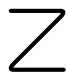
\includegraphics[keepaspectratio]{images/part002_15bf1a92.jpg}}

注. 注意两个等价的 (H) 函数可以有不等价的反函数，如两个函数 \(\log x\) 与 \(1 + \log x\) 的例子所示。

\setcounter{exercisegroup}{0}
\refstepcounter{exercisegroup}
\section*{第 \S\arabic{exercisegroup} 节习题}
\phantomsection
\addcontentsline{toc}{section}{第 \protect\S\arabic{exercisegroup} 节习题}

\begin{enumerate}
\def\labelenumi{\arabic{enumi})}
\tightlist
\item
  证明：对实变量 \(x\) （趋于 \(+\infty\) ），函数
\end{enumerate}

\[
f (x) = \left(x \cos^ {2} x + \sin^ {2} x\right) e ^ {x ^ {2}}
\]

单调，但它既不与 \(e^{x^2}\) 可比较，也不与 \(x^{1/2}e^{x^2}\) 弱可比较。

\begin{enumerate}
\def\labelenumi{\arabic{enumi})}
\setcounter{enumi}{1}
\tightlist
\item
  设 \(\varphi\) 是一个严格正的函数，对 \(x > 0\) 有定义且递增，并满足 \(\varphi \gg 1\) 。
\end{enumerate}

\begin{enumerate}
\def\labelenumi{\alph{enumi})}
\item
  证明：若函数 \(\log \varphi(x) / \log x\) 递增，则函数之间的关系 \(f \ll g\) （这些函数 \(>0\) ）蕴含 \(\varphi \circ f \ll \varphi \circ g\) （当 \(g \gg 1\) 时）。
\item
  给出一个例子，其中 \(\log \varphi(x)/\log x\) 递减，f 与 g 是两个 \textgreater0 的函数，满足 \(g \gg 1\) 且 \(f \sim g\) ，但 \(\varphi \circ f\) 不等价于 \(\varphi \circ g\) 。
\end{enumerate}

3) a) 设 \((\alpha_{i},\beta_{i})\) 是 \(n\) 个互异的实数对（由实数 \(\geqslant 0\) 组成），异于 \((0,0)\) ，且满足 \(\inf_{i}\alpha_{i} = \inf_{i}\beta_{i} = 0\) 。考察方程

\[
f (x, y) = \sum_ {i = 1} ^ {n} a _ {i} x ^ {\alpha_ {i}} y ^ {\beta_ {i}} \left(1 + \varphi_ {i} (x, y)\right) = 0
\]

其中诸 \(a_{i}\) 是 \(\neq0\) 的实数，诸 \(\varphi_{i}\) 是正方形 \(0\leqslant x\leqslant a,0\leqslant y\leqslant a\) 上的连续函数，且当 \((x,y)\) 趋于 \((0,0)\) 时趋于 0。假设存在一个函数 g，它在区间 {[}0,b{]} 上为正且连续，随 x 趋于 0，且满足 \(f(x,g(x))=0\) （对所有 \(x\in[0,b]\) ）。证明：对每个实数 \(\mu>0\) ，当 x 趋于 0 时 \(g(x)/x^{\mu}\) 趋于一个有限或无穷的极限（利用 V, p.~217, prop. 9，对每个数 \(t\geqslant0\) 考察方程 \(f(x,tx^{\mu})=0\) ）。

\begin{enumerate}
\def\labelenumi{\alph{enumi})}
\setcounter{enumi}{1}
\item
  为使 \(g(x)/x^{\mu}\) 趋于一个有限极限 \(\neq0\) ，必须 \(\mu\) 满足：至少存在两个互异的对 \((\alpha_{h},\beta_{h})\) 与 \((\alpha_{k},\beta_{k})\) ，使 \(\alpha_{h}+\mu\beta_{h}=\alpha_{k}+\mu\beta_{k}\) ，且对每个其余的对 \((\alpha_{i},\beta_{i})\) 有 \(\alpha_{i}+\mu\beta_{i}\geqslant\alpha_{h}+\mu\beta_{h}\) 。这样就得到有限多个可能的值 \(\mu_{j}(1\leqslant j\leqslant r)\) ；数 \(-1/\mu_{j}\) 是平面 \(R^{2}\) 中这样的仿射直线的斜率：这些直线至少包含点集 \((\alpha_{i},\beta_{i})\) 中的两个点，且该点集的其余各点都位于所考虑的直线上方（“牛顿多边形”）。
\item
  设 \(\mu_{1}\) 是诸数 \(\mu_{j}\) 中最小者。证明 \(g(x) / x^{\mu_1}\) 趋于一个有限极限（可能为零）。（首先证明总可假定：若 \(i\) 与 \(j\) 是两个互异的指标，则不能同时有 \(\alpha_{i} \leqslant \alpha_{j}\) 与 \(\beta_{i} \leqslant \beta_{j}\) ；由此推出可设 \(\alpha_{1} = 0\) ， \(\alpha_{i} > 0\) 与 \(\beta_{i} < \beta_{1}\) （对 \(i \neq 1\) ）；然后令 \(g(x) = t(x)x^{\mu_1}\) ，证明 \(t(x)\) 不能趋于 \(+\infty\) （当 \(x\) 趋于 0）。）
\end{enumerate}

\(d)\) 由 \(c\) ) 出发，对 \(r\) 作递归，推出存在一个指标 \(j\) ，使 \(g(x) / x^{\mu_j}\) 趋于一个有限极限 \(\neq 0\) （当 \(x\) 趋于 0）。

\setcounter{exercisegroup}{2}
\refstepcounter{exercisegroup}
\section*{第 \S\arabic{exercisegroup} 节习题}
\phantomsection
\addcontentsline{toc}{section}{第 \protect\S\arabic{exercisegroup} 节习题}

\begin{enumerate}
\def\labelenumi{\arabic{enumi})}
\item
  定义一个递增函数 \(g\) ，它在 \(+\infty\) 的某个邻域上有连续导数，使 \(g\) 与 \(1 / x\) 可比较到 1 阶，但 \(x\) 与 \(1 / g\) 不可比较到 1 阶（取 \(g'(x) = 1\) ，但在以点 \(x = n\) （ \(n\) 为整数 \(>0\) ）为中心的充分小区间上 \(g'\) 取非常大的值）。
\item
  设 f 与 g 是两个 \(\geqslant0\) 的函数（随 x 趋于 \(+\infty\) ），且可比较到 1 阶；若 h 是一个可导函数， \(\geqslant0\) 且递增（当 x 趋于 \(+\infty\) ），证明 hf 与 hg 可比较到 1 阶。
\item
  给出两个函数的例子：它们为正、递减、当 x 趋于 \(+\infty\) 时趋于 0、可比较到 1 阶，且使 \(xf(x)\) 与 \(xg(x)\) 不可比较到 1 阶（取 f 与 g 等价，且使
\end{enumerate}

\[
\frac {f ^ {\prime} (x)}{f (x)} + \frac {1}{x} \qquad \text { and } \qquad \frac {g ^ {\prime} (x)}{g (x)} + \frac {1}{x}
\]

不可比较）。

\begin{enumerate}
\def\labelenumi{\arabic{enumi})}
\setcounter{enumi}{3}
\tightlist
\item
  \begin{enumerate}
  \def\labelenumii{\alph{enumii})}
  \tightlist
  \item
    证明 \(\frac{\sin x}{\sqrt{x}} \sim \frac{\sin x}{\sqrt{x}} \left(1 + \frac{\sin x}{\sqrt{x}}\right)\) ，但积分 \(\int_{a}^{+\infty} \frac{\sin t}{\sqrt{t}} dt\) 收敛，而积分 \(\int_{a}^{+\infty} \frac{\sin t}{\sqrt{t}} \left(1 + \frac{\sin t}{\sqrt{t}}\right) dt\) 为无穷。
  \end{enumerate}
\end{enumerate}

\begin{enumerate}
\def\labelenumi{\alph{enumi})}
\setcounter{enumi}{1}
\item
  证明积分 \(\int_{a}^{+\infty}\frac{\sin t}{t}dt\) 与 \(\int_{a}^{+\infty}\frac{\sin^{2}t}{t^{2}}dt\) 都收敛，但 \(\int_{x}^{+\infty}\frac{\sin^{2}t}{t^{2}}dt\) 相对于 \(\int_{x}^{+\infty}\frac{\sin t}{t}dt\) 并非可忽略，尽管 \(\sin^{2}t/t^{2}\ll\sin t/t\) 。
\item
  考虑取值于 \(R^{2}\) 的两个连续函数（定义在 \([1, +\infty[\) 上）：
\end{enumerate}

\[
\mathbf {f}: x \mapsto \left(\frac {1}{x ^ {2}}, \frac {\sin x}{x}\right), \quad \mathbf {g}: x \mapsto \left(\frac {1}{x ^ {2}}, \frac {\sin x}{x} \left(1 + \frac {\sin x}{x}\right)\right).
\]

证明它们对 \(x\) 的任何值都不为零， \(\mathbf{f} \sim \mathbf{g}\) （当 \(x\) 趋于 \(+\infty\) 时），积分 \(\int_{a}^{+\infty} \mathbf{f}(t) dt\) 与 \(\int_{a}^{+\infty} \mathbf{g}(t) dt\) 收敛，但 \(\int_{x}^{+\infty} \mathbf{f}(t) dt\) 不等价于 \(\int_{x}^{+\infty} \mathbf{g}(t) dt\) （当 \(x\) 趋于 \(+\infty\) 时）。

5) 设 \(f\) 是定义在 \(+\infty\) 的某个邻域上的实凸函数，且满足 \(f(x) \gg x\) 。称 \(f\) 在 \(+\infty\) 的某个邻域上是正则凸的，如果对每个凸函数 \(g\) （定义在 \(+\infty\) 的某个邻域上）且满足 \(f \sim g\) ，也有 \(f_d' \sim g_r'\) 。

对每个数 \(\alpha > 0\) 与充分大的 x，设 \(k(\alpha, x)\) 是诸数 \(\left(f(y) - (y - x)f_{d}'(y)\right)/f(x)\) 的下确界（当 y 取遍 \(\geqslant x\) 且满足 \(f_{d}'(y) \leqslant (1 + \alpha)f_{d}'(x)\) 的数所成的集时）。类似地，设 \(h(\alpha, x)\) 是诸数

\[
\left(f (z) + (x - z) f _ {d} ^ {\prime} (z)\right) / f (x)
\]

（当 \(z\) 取遍 \(\leqslant x\) 且满足 \(f_d'(z) \geqslant (1 - \alpha)f_d'(x)\) 的数所成的集时）的下确界。设 \(\psi(\alpha) = \limsup_{x \to +\infty} k(\alpha, x)\) ， \(\varphi(\alpha) = \limsup_{x \to +\infty} h(\alpha, x)\) 。证明： \(f\) 在

\(+\infty\) 的某个邻域上正则凸的充分必要条件是，对一切充分小的 \(\alpha\) 有 \(\psi(\alpha) < 1\) 且 \(\varphi(\alpha) < 1\) 。

6) 设 \(\mathbf{f}\) 是某个区间 \([x_0, +\infty[\) （属于 \(\mathbf{R}\) ）上的连续向量函数，且对所有 \(\lambda \geqslant 0\) ，函数 \(\mathbf{f}(x + \lambda) - \mathbf{f}(x)\) 当 \(x\) 趋于 \(+\infty\) 时趋于 0。

\begin{enumerate}
\def\labelenumi{\alph{enumi})}
\tightlist
\item
  证明： \(\mathbf{f}(x+\lambda)-\mathbf{f}(x)\) 当 \(\lambda\) 属于任一紧区间 \(K=[a,b]\) （ \([0,+\infty[\) 中的）时随 1/x 一致地趋于 0。（用反证法：若存在一个序列 \((x_{n})\) 趋于 \(+\infty\) ，以及 K 中的点列 \((\lambda_{n})\) 使
\end{enumerate}

\[
\| \mathbf {f} (x _ {n} + \lambda_ {n}) - \mathbf {f} (x _ {n}) \| > \alpha > 0
\]

对每个 n 成立，则存在 \(J_{n}\) （ \(\lambda_{n}\) 在 K 中的一个邻域），使对每个 \(\lambda \in J_{n}\) 有 \(\|\mathbf{f}(x_{n} + \lambda) - \mathbf{f}(x_{n})\| > \alpha\) 。用归纳法构造一个递减的闭区间序列 \(I_{k} \subset K\) 与一个子序列 \((x_{n_{k}})\) （ \((x_{n})\) 的），使 \(\|\mathbf{f}(x_{n_{k}} + \lambda) - \mathbf{f}(x_{n_{k}})\| \geqslant \alpha/3\) 对每个 \(\lambda \in I_{k}\) 成立；为此注意，若 \(\delta_{k}\) 是 \(I_{k}\) 的长度而 q 是使 \(q\delta_{k} > b - a\) 的整数，则只要 x 充分大就有 \(\|\mathbf{f}(x + \delta_{k}) - \mathbf{f}(x)\| \leqslant \alpha/3q\) 。）

\begin{enumerate}
\def\labelenumi{\alph{enumi})}
\setcounter{enumi}{1}
\tightlist
\item
  由 \(a\) ) 推出 \(\int_{x}^{x + 1}\mathbf{f}(t)dt - \mathbf{f}(x)\) 当 \(x\) 趋于 \(+\infty\) 时趋于 0，并断定 \(\mathbf{f}(x) = o(x)\) 。
\end{enumerate}

\begin{enumerate}
\def\labelenumi{\arabic{enumi})}
\setcounter{enumi}{6}
\tightlist
\item
  设 g 是一个严格正的实函数，在某个区间 \([x_{0}, +\infty[\) 上连续，且对每个 \(\mu > 0\) 有 \(g(\mu x) \sim g(x)\) 。由习题 6 推出 g 相对于 x 的阶为 0。
\end{enumerate}

\setcounter{exercisegroup}{3}
\refstepcounter{exercisegroup}
\section*{第 \S\arabic{exercisegroup} 节习题}
\phantomsection
\addcontentsline{toc}{section}{第 \protect\S\arabic{exercisegroup} 节习题}

\begin{enumerate}
\def\labelenumi{\arabic{enumi})}
\item
  若通项为 \(u_{n} \geqslant 0\) 的级数收敛，则通项为 \(\sqrt{u_n u_{n+1}}\) 的级数也收敛。逆命题一般不成立；证明当级数 \((u_n)\) 递减时逆命题成立。
\item
  设 \((p_{n})\) 是一个递增的数 \textgreater{} 0 的序列（趋于 \(+\infty\) ）。
\end{enumerate}

\begin{enumerate}
\def\labelenumi{\alph{enumi})}
\tightlist
\item
  若比值 \(p_n / p_{n-1}\) 当 \(n\) 无限增大时趋于 1，证明
\end{enumerate}

\[
\sum_ {k = 1} ^ {n} \frac {p _ {k} - p _ {k - 1}}{p _ {k}} \sim \log p _ {n}
\]

\[
\sum_ {k = 1} ^ {n} p _ {k} ^ {\rho} (p _ {k} - p _ {k - 1}) \sim \frac {1}{\rho + 1} p _ {n} ^ {\rho + 1} \quad \text { for } \rho > - 1
\]

（应用 V, p.~237 的命题 2）。

\begin{enumerate}
\def\labelenumi{\alph{enumi})}
\setcounter{enumi}{1}
\item
  不对比值 \(p_{n}/p_{n-1}\) 作假设，证明通项为 \((p_{n}-p_{n-1})/p_{n}\) 的级数总有无穷和（区分 \(p_{n}/p_{n-1}\) 趋于 1 与不趋于 1 两种情形）。
\item
  证明对每个 \(\rho > 0\) ，通项为 \((p_n - p_{n-1}) / p_n p_{n-1}^\rho\) 的级数收敛（与通项为 \(\frac{1}{p_{n-1}^\rho} - \frac{1}{p_n^\rho}\) 的级数比较）。
\end{enumerate}

\begin{enumerate}
\def\labelenumi{\arabic{enumi})}
\setcounter{enumi}{2}
\item
  证明：对每个收敛级数 \((u_{n})\) （项 \(>0\) ），存在一个级数 \((v_{n})\) （具有无穷和、项 \(>0\) ），使 \(\liminf v_n / u_n = 0\) 。
\item
  设 \((u_{n})\) 是一个递减的数 \textgreater0 的序列；若存在一个整数 k，使从某个 n 起 \(ku_{kn} \geqslant u_{n}\) 对一切 n 成立，则通项为 \(u_{n}\) 的级数有无穷和。
\item
  设 \((u_{n})\) 是一个从某项起项 \(>0\) 的级数。证明：若
\end{enumerate}

\[
\operatorname * {l i m s u p} _ {n \to \infty} \left(\frac {u _ {n + 1}}{u _ {n}}\right) ^ {n} <   \frac {1}{e}
\]

则级数收敛；若 \(\liminf_{n\to\infty}\left(\frac{u_{n+1}}{u_n}\right)^n\geqslant\frac{1}{e}\) ，则级数有无穷和。

\begin{enumerate}
\def\labelenumi{\arabic{enumi})}
\setcounter{enumi}{5}
\item
  设 \((u_{n})\) 是由 \(\neq 0\) 的实数组成的级数，且 \(\lim_{n\to \infty}u_n = 0\) 。证明：若存在一个数 \(r\) 满足 \(0 < r < 1\) ，且从某个 n 起有 \(-1\leqslant u_{n + 1} / u_n\leqslant r\) ，则级数 \((u_{n})\) 收敛。
\item
  设 \((u_{n})\) 是一个项 \(>0\) 的收敛级数。
\end{enumerate}

\begin{enumerate}
\def\labelenumi{\alph{enumi})}
\tightlist
\item
  证明
\end{enumerate}

\[
\lim _ {n \rightarrow \infty} \frac {u _ {1} + 2 u _ {2} + \cdots + n u _ {n}}{n} = 0.
\]

\begin{enumerate}
\def\labelenumi{\alph{enumi})}
\setcounter{enumi}{1}
\tightlist
\item
  证明
\end{enumerate}

\[
\sum_ {n = 1} ^ {\infty} \frac {u _ {1} + 2 u _ {2} + \cdots + n u _ {n}}{n (n + 1)} = \sum_ {n = 1} ^ {\infty} u _ {n}
\]

\[
\left(\text { write } \frac {1}{n (n + 1)} = \frac {1}{n} - \frac {1}{n + 1}\right).
\]

\begin{enumerate}
\def\labelenumi{\alph{enumi})}
\setcounter{enumi}{2}
\tightlist
\item
  由 a) 与 b) 推出
\end{enumerate}

\[
\lim _ {n \to \infty} n (u _ {1} u _ {2} \dots u _ {n}) ^ {1 / n} = 0
\]

以及

\[
\sum_ {n = 1} ^ {\infty} \frac {(n ! u _ {1} u _ {2} \dots u _ {n}) ^ {1 / n}}{n + 1} <   \sum_ {n = 1} ^ {\infty} u _ {n}
\]

（应用 III, p.~93 的不等式 (8)）。

8) a) 设 \((z_{n})\) 是一个复数序列。证明：若通项分别为 \(z_{n}, z_{n}^{2}, \ldots, z_{n}^{q-1}, |z_{n}|^{q}\) 的级数都收敛，则通项因子为 \(1 + z_{n}\) 的无穷乘积收敛。

\begin{enumerate}
\def\labelenumi{\alph{enumi})}
\setcounter{enumi}{1}
\tightlist
\item
  若 \(z_{n}\) 是实数且通项为 \(z_{n}\) 的级数收敛，则通项因子为 \(1 + z_{n}\) 的无穷乘积在通项为 \(z_{n}^{2}\) 的级数收敛时收敛，且有
\end{enumerate}

\[
\underset {n = 1} {\overset {\infty} {\mathrm{P}}} (1 + z _ {n}) = 0 \quad \text { if } \quad \sum_ {n = 1} ^ {\infty} z _ {n} ^ {2} = + \infty .
\]

\begin{enumerate}
\def\labelenumi{\alph{enumi})}
\setcounter{enumi}{2}
\tightlist
\item
  对每个整数 \(p \geqslant 2\) 令
\end{enumerate}

\[
k _ {p} = [ \log \log p ], \quad h _ {p} = \sum_ {j = 1} ^ {p - 1} k _ {j}, \quad \omega_ {p} = \frac {2 \pi}{k _ {p}}.
\]

按下述方式定义复数序列 \((z_{n})\) ：对 \(n = h_{p} + m\) ， \(0 \leqslant m \leqslant k_{p} - 1\) ，令 \(z_{n} = e^{mi\omega_{p}} / \log p\) 。证明对每个整数 q \textgreater{} 0，通项为 \(z_{n}^{q}\) 的级数收敛，但通项因子为 \(1 + z_{n}\) 的乘积不收敛。

\begin{enumerate}
\def\labelenumi{\arabic{enumi})}
\setcounter{enumi}{8}
\tightlist
\item
  \begin{enumerate}
  \def\labelenumii{\alph{enumii})}
  \tightlist
  \item
    借助斯特林公式证明：函数 \(f_{n}(x) = \left|e^{-2x} - e^{-x}\sum_{k=0}^{n}(-1)^{k}\frac{x^{k}}{k!}\right|\) 在区间 \([0, +\infty[\) 上的最大值随 \(1/n\) 趋于 0。
  \end{enumerate}
\end{enumerate}

\begin{enumerate}
\def\labelenumi{\alph{enumi})}
\setcounter{enumi}{1}
\tightlist
\item
  由 a) 出发对整数 p 作归纳推出：对每个 \(\varepsilon > 0\) 存在一个多项式 \(g(x)\) ，使 \(\left|e^{-px} - e^{-x}g(x)\right| \leqslant \varepsilon\) 对每个 \(x \geqslant 0\) 成立（在 a) 中把 x 换成 px/2，并对 \(e^{-(p-1)x/2}\) 应用归纳假设）。
\end{enumerate}

\begin{enumerate}
\def\labelenumi{\arabic{enumi})}
\setcounter{enumi}{9}
\tightlist
\item
  对每个数 \(\alpha > 0\) 推出公式
\end{enumerate}

\[
1 ^ {\alpha n} + 2 ^ {\alpha n} + \dots + n ^ {\alpha n} \sim \frac {n ^ {\alpha n}}{1 - e ^ {- \alpha}}
\]

其中 n 趋于 \(+\infty\) 。

11) 对每个数 \(\alpha > 0\) 推出公式

\[
(1!) ^ {- \alpha / n} + (2!) ^ {- \alpha / n} + \dots + (n!) ^ {- \alpha / n} \sim \frac {1}{\alpha} \frac {n}{\log n}
\]

其中 \(n\) 趋于 \(+\infty\) （把每一项 \((p!)^{-\alpha / n}\) 与 \(n^{-\alpha p / n}\) 比较）。

\section*{附录习题}
\phantomsection
\addcontentsline{toc}{section}{附录习题}

\begin{enumerate}
\def\labelenumi{\arabic{enumi})}
\tightlist
\item
  设 \(\mathfrak{K}\) 是一个哈代域，使得对每个函数 \(f\in \mathfrak{K}\) （在 \(+\infty\) 的某个邻域上不恒为零）存在一个 \(\lambda >0\) 使
\end{enumerate}

\[
\frac {1}{e _ {m} (x ^ {\lambda})} \ll f (x) \ll e _ {m} (x ^ {\lambda})
\]

（m 是一个与 f 无关的整数）。

\begin{enumerate}
\def\labelenumi{\alph{enumi})}
\tightlist
\item
  设 \(u_{1}, u_{2}, \ldots, u_{p}\) 是 p 个形如 \(u_{k} = \log |z_{k}|\) 的函数，其中 \(z_{k} \in K\) 在 \(+\infty\) 的某个邻域上不为零。证明：对每个函数 g（在 \(+\infty\) 的某个邻域上不为零；属于哈代域 \(\mathfrak{K}(u_{1}, u_{2}, \ldots, u_{p})\) ，该域由把诸函数 \(u_{k}\) （ \(1 \leqslant k \leqslant p\) ）添加到 K 而得到），存在一个数 \(\mu > 0\) 使
\end{enumerate}

\[
\frac {1}{e _ {m} (x ^ {\mu})} \ll g (x) \ll e _ {m} (x ^ {\mu})
\]

（归结为 g 是系数在 K 中的 \(u_{k}\) 的多项式的情形，对 p 作归纳论证；然后对 p = 1，仿照 V, p.~248 引理 2 的做法对多项式 g 的次数作归纳论证）。

\begin{enumerate}
\def\labelenumi{\alph{enumi})}
\setcounter{enumi}{1}
\tightlist
\item
  设 \(u_{k}\) （ \(1 \leqslant k \leqslant p\) ）是 \(p\) 个形如 \(u_{k} = \exp(z_{k})\) 的函数，其中 \(z_{k} \in \mathcal{K}\) 。证明：对每个函数 \(g\) （属于哈代域 \(\mathcal{K}(u_{1}, u_{2}, \ldots, u_{p})\) ，在 \(+\infty\) 的某个邻域上不恒为零），存在一个数 \(\mu > 0\) 使
\end{enumerate}

\[
\frac {1}{e _ {m + 1} (x ^ {\mu})} \prec g (x) \prec e _ {m + 1} (x ^ {\mu})
\]

（类似的方法）。

\begin{enumerate}
\def\labelenumi{\alph{enumi})}
\setcounter{enumi}{2}
\tightlist
\item
  推出：若 \(f\) 是一个具有 \(n\) 项定义序列、且在 \(+\infty\) 的某个邻域上不恒为零的 (H) 函数，则存在一个数 \(\lambda > 0\) 使
\end{enumerate}

\[
\frac {1}{e _ {n} (x ^ {\lambda})} \ll f (x) \ll e _ {n} (x ^ {\lambda}).
\]

\begin{enumerate}
\def\labelenumi{\arabic{enumi})}
\setcounter{enumi}{1}
\tightlist
\item
  \begin{enumerate}
  \def\labelenumii{\alph{enumii})}
  \tightlist
  \item
    证明每个只有一项定义序列的 (H) 函数等价于形如 \(x^{p}(\log x)^{q}\) 或 \(x^{p}e^{g(x)}\) 之一的函数，其中 p 与 q 是有理整数，g 是 x 的多项式（习题 1 的方法）。
  \end{enumerate}
\end{enumerate}

\begin{enumerate}
\def\labelenumi{\alph{enumi})}
\setcounter{enumi}{1}
\tightlist
\item
  由 a) 推出：哈代域 \(\mathbf{R}(x,u_{1},\ldots,u_{p})\) （其中 \(u_{1},\ldots,u_{p}\) 是只有单项定义序列的 (H) 函数）中每个函数都等价于形如 \(x^{p}(\log x)^{q}e^{g(x)}\) 的函数，其中 p 与 q 是有理整数，g 是 x 的多项式。
\end{enumerate}

\begin{enumerate}
\def\labelenumi{\arabic{enumi})}
\setcounter{enumi}{2}
\item
  设 f 与 g 是两个 (H) 函数，使 f/g 相对于 \(l_{m}(x)\) 的阶为 0；证明：若 g 相对于 \(l_{m}(x)\) 的阶不为 0，则 \(f'/g' \sim f/g\) （比较 \(\log |f|\) 与 \(\log |g|\) ）。
\item
  设 \(\mathfrak{K}\) 是一个哈代域，使得对每个函数 \(f\in \mathfrak{K}\) （不等价于常数、且相对于 \(l_{m - 1}(x)\) 的阶为 0），存在一个常数 \(k\) 与一个有理整数 \(r\) ，使 \(f(x)\sim k(l_m(x))^r\) 。
\end{enumerate}

\begin{enumerate}
\def\labelenumi{\alph{enumi})}
\item
  设 z 是 K 中任一在 \(+\infty\) 的某个邻域上不恒为零的函数。证明：哈代域 \(\mathcal{K}(\log|z|)\) 中每个不等价于常数、且相对于 \(l_{m}(x)\) 的阶为 0 的函数 g，都等价于形如 \(k(l_{m+1}(x))^{r}\) 的函数（k 为常数，r 为有理整数）。（先考虑 g 是 \(\log|z|\) 的 p 次多项式、系数在 K 中的情形，并用习题 3 对 p 作归纳论证；若 g 是 \(\log|z|\) 的有理函数、系数在 K 中，则用习题 3 对分子的次数作归纳论证。）
\item
  证明 \(\mathfrak{K}(l_{m+1}(x))\) 中每个函数都等价于形如 \(f(x)(l_{m+1}(x))^r\) 的函数，其中 \(f \in \mathfrak{K}\) ， \(r\) 是有理整数。
\item
  设 z 是 K 中任一函数。证明：哈代域 \(\mathfrak{K}(e^{z})\) 中每个相对于 \(l_{m}(x)\) 的阶为 0 的函数 g 都等价于一个常数。（先考虑 \(g = u^{q} \mathrm{P}(u)\) 的情形，其中 \(u = e^{z}\) ，q 是有理整数， \(\mathrm{P}(u)\) 是 u 的 p 次多项式、系数在 K 中；然后用 a) 与习题 3 对 p 作归纳论证。再用习题 3 过渡到一般情形。）
\item
  把 a) 的结果推广到域 \(\mathfrak{K}(u_{1}, u_{2}, \ldots, u_{s})\) ，其中诸 \(u_{k}\) 形如 \(e^{z_{k}}\) 或 \(\log |z_{k}|\) ，诸 \(z_{k}\) 是 K 中在 \(+\infty\) 的某个邻域上不恒为零的函数（对 s 作归纳论证）。
\end{enumerate}

\begin{enumerate}
\def\labelenumi{\arabic{enumi})}
\setcounter{enumi}{4}
\tightlist
\item
  \begin{enumerate}
  \def\labelenumii{\alph{enumii})}
  \tightlist
  \item
    由习题 4 推出：若 f 是一个具有 n 项定义序列、不等价于常数、且相对于 \(l_{n-1}(x)\) 的阶为 0 的 (H) 函数，则存在一个常数 k 与一个有理整数 r，使 \(f(x) \sim k(l_n(x))^r\) 。
  \end{enumerate}
\end{enumerate}

\begin{enumerate}
\def\labelenumi{\alph{enumi})}
\setcounter{enumi}{1}
\tightlist
\item
  由习题 4 推出：若 \(f\) 是任一 (H) 函数，则存在一个整数 \(n\) ，使 \(n\) 阶对数判别法能够判定积分 \(\int_{a}^{+\infty} f(t) dt\) 收敛或为无穷。
\end{enumerate}

\begin{enumerate}
\def\labelenumi{\arabic{enumi})}
\setcounter{enumi}{5}
\tightlist
\item
  把函数 \(e_p\left((l_q(x))^{\mu}\right)\) 按整数 \(p\) 与 \(q\) 以及实数 \(\mu\) （设其 \(> 0\) 且 \(\neq 1\) ）的取值相互比较。
\end{enumerate}

7) 设 \(f\) 是一个具有 \(n\) 项定义序列的 (H) 函数。证明：若有 \(e_p((l_{q+1}(x))^{\beta}) \ll f(x) \ll e_p((l_q(x))^{\alpha})\) （相应地， \(e_p((l_q(x))^{\beta}) \ll f(x) \ll e_{p+1}((l_q(x))^{\alpha}))\) ），

则对每个 \(\beta > 0\) 与每个 \(\alpha\) （ \(0 < \alpha < 1\) ），必有 \(p + q + 1 < n\) （对 \(n\) 作归纳论证，使用与习题 1 (V, p.~263) 和 4 (V, p.~264) 类似的方法）。

\begin{enumerate}
\def\labelenumi{\arabic{enumi})}
\setcounter{enumi}{7}
\tightlist
\item
  \begin{enumerate}
  \def\labelenumii{\alph{enumii})}
  \tightlist
  \item
    设 \((f_{n})\) 是属于 \(\mathcal{H}(\mathfrak{F},\mathbf{R})\) 的递增连续函数序列，且对每个 n 有 \(f_{n} \ll f_{n+1}\) 。证明存在一个连续、递增、属于 \(\mathcal{H}(\mathfrak{F},\mathbf{R})\) 的函数 f，使对每个 n 有 \(f \gg f_{n}\) （归结为 \(f_{n} \leqslant f_{n+1}\) 的情形，并定义 f 使 \(f_{n}(x) \leqslant f(x) \leqslant f_{n+1}(x)\) （对 \(n \leqslant x \leqslant n+1\) ））。
  \end{enumerate}
\end{enumerate}

\begin{enumerate}
\def\labelenumi{\alph{enumi})}
\setcounter{enumi}{1}
\item
  设 \((f_n)\) 是属于 \(\mathcal{H}(\mathfrak{F},\mathbf{R})\) 的递增连续函数序列，且 \(1\ll f_{n + 1}\ll f_n\) 对每个 \(n\) 成立。证明存在一个函数 \(f\) ，连续、递增、属于 \(\mathcal{H}(\mathfrak{F},\mathbf{R})\) ，使 \(1\ll f\ll f_n\) 对每个 \(n\) 成立（归结为 \(f_{n + 1}\leqslant f_n\) 的情形，并证明可以定义一个递增的实数序列 \((x_{n})\) 与一个连续递增函数 \(f\) ，使 \(f_{n + 1}(x)\leqslant f(x)\leqslant f_n(x)\) （对 \(x_{n}\leqslant x\leqslant x_{n + 1}\) ））。
\item
  设 \((f_n), (g_n)\) 是两个属于 \(\mathcal{H}(\mathfrak{F}, \mathbf{R})\) 的连续递增函数序列，满足 \(f_n \ll f_{n+1}\) 、 \(g_m \gg g_{m+1}\) 且 \(f_n \ll g_m\) （对所有 \(m\) 与 \(n\) ）；证明存在一个函数 \(h\) ，连续、递增、属于 \(\mathcal{H}(\mathfrak{F}, \mathbf{R})\) ，使 \(f_n \ll h \ll g_m\) （对所有 \(m\) 与 \(n\) ）（类似的方法）。
\end{enumerate}

特别地，证明存在一个连续递减函数 \(f\) （属于 \(\mathcal{H}(\mathfrak{F},\mathbf{R})\) ），使任何对数判别法都不能判定积分 \(\int_{a}^{+\infty}f(t)dt\) 收敛或为无穷（“杜·布瓦–雷蒙定理”）。

\begin{enumerate}
\def\labelenumi{\arabic{enumi})}
\setcounter{enumi}{8}
\item
  证明级数 \(\sum_{n=1}^{\infty} \frac{e_n(x)}{e_n(n)}\) 在 \(\mathbf{R}\) 的每个紧子集上一致收敛，且其和 \(f(x)\) 满足： \(f(x) \gg e_n(x)\) 对每个整数 \(n\) 成立。
\item
  证明存在一个递增函数 \(f\) ，它有定义、连续且 \(> 0\) （对 \(x \geqslant 0\) ），使 \(f(2x) = 2^{f(x)}\) 对所有 \(x \geqslant 0\) 成立；由此推出 \(f(x) \gg e_n(x)\) 对每个整数 \(n\) 成立。
\item
  设 \(f\) 是一个递增函数，连续且 \(\geqslant 0\) （对 \(x \geqslant 0\) 有定义），且 \(f(x) \gg e_n(x)\) 对每个整数 \(n\) 成立；证明：若 \(g\) 是 \(f\) 的反函数，则 \(1 \ll g(x) \ll l_n(x)\) 对每个整数 \(n\) 成立。
\end{enumerate}

12) 对每个整数 \(n > 0\) ，设 \(n = \sum_{k=0}^{\infty} \varepsilon_k 2^k\) 是 \(n\) 的二进展开（ \(\varepsilon_k\) 是整数，除有限个指标外均为零， \(0 \leqslant \varepsilon_k \leqslant 1\) ）。令

\[
\alpha (n) = \sum_ {k = 0} ^ {\infty} \varepsilon_ {k}, \quad \mathrm{A} _ {1} (n) = \sum_ {j = 1} ^ {n} \alpha (j), \quad \mathrm{A} _ {2} (n) = \sum_ {j = 1} ^ {n} \alpha (\alpha (j)).
\]

\begin{enumerate}
\def\labelenumi{\alph{enumi})}
\tightlist
\item
  证明公式 \(\mathrm{A}_1(n) = \sum_{k=0}^{\infty}(k+2)\varepsilon_k 2^{k-1}\) 。由此推出公式
\end{enumerate}

\[
\mathrm{A} _ {1} (n) = \frac {n}{2} \frac {\log n}{\log 2} + o (n \log \log n)
\]

其中 \(n\) 无限增大（把表示 \(\mathrm{A}_1(n)\) 的和分解成两部分：第一个和中指标 \(k\) 从 0 变到 \(\mu(n)\) ，第二个和中从 \(\mu(n)\) 变到 \(n_1\) ，这里 \(n_1\) 是数 \(k\) （使 \(\varepsilon_k \neq 0\) ）中最大者，而 \(\mu(n)\) 取得适当；用 V, p.~239 的命题 6 估计第一个和的上界，然后估计第二个和与 \(n_1n / 2\) 之差。

\begin{enumerate}
\def\labelenumi{\alph{enumi})}
\setcounter{enumi}{1}
\tightlist
\item
  建立关系式
\end{enumerate}

\[
\sum_ {j = 0} ^ {2 ^ {m} - 1} f (\alpha (j)) = \sum_ {k = 0} ^ {m} \binom {m} {k} f (k)
\]

其中 \(f\) 是定义在 \(\mathbf{N}\) 上的任意函数（对给定的 \(k\) ，考察 \(j < 2^{m}\) 中使 \(\alpha(j) = k\) 的个数）。

\begin{enumerate}
\def\labelenumi{\alph{enumi})}
\setcounter{enumi}{2}
\tightlist
\item
  对 \(m = 2^r - 1\) ，证明 \(\alpha(m - j) + \alpha(j) = r\) 。由此并借助 \(b\) ) 推出
\end{enumerate}

\[
\mathrm{A} _ {2} (2 ^ {m}) = r 2 ^ {m - 1} \sim \frac {2 ^ {m} \log \log 2 ^ {m}}{2 \log 2}.
\]

\begin{enumerate}
\def\labelenumi{\alph{enumi})}
\setcounter{enumi}{3}
\tightlist
\item
  对 \(m = 2^{r}\) ，证明
\end{enumerate}

\[
\mathrm{A} _ {2} (2 ^ {m}) = 2 \mathrm{A} _ {2} (2 ^ {m - 1}) + 2 ^ {m - 1} - \sum_ {j = 0} ^ {m - 1} \binom {m - 1} {j} \Delta (j + 1)
\]

其中我们令 \(\alpha(n+1)-\alpha(n)=1-\Delta(n+1)\) （对所有 \(n\) ；利用 \(b\) ）以及关系式 \(\alpha(2^{k}+r)=\alpha(r)+1\) （对 \(r<2^{k}\) ））。证明 \(\sum_{j=0}^{m-1}\binom{m-1}{j}\Delta(j+1)\leqslant r^{m-2}\) （注意 \(\Delta(j+1)=0\) （若 \(j\) 为偶数），且 \(\Delta(j+1)\leqslant\log j/\log 2\) 对所有 \(j\) 成立）。借助 \(c\) ) 推出

\[
\mathrm{A} _ {2} (2 ^ {m}) \geqslant \frac {3}{2} r 2 ^ {m - 1} \geqslant \frac {3}{2} \frac {2 ^ {m} \log \log 2 ^ {m}}{2 \log 2}.
\]

由 \(c\) ) 与这个关系式断定： \(\mathrm{A}_2(n)\) 当 \(n\) 趋于 \(+\infty\) 时不等价于任何 (H) 函数。

\begin{enumerate}
\def\labelenumi{\arabic{enumi})}
\setcounter{enumi}{12}
\tightlist
\item
  设 \(f\) 是一个满足 \(1 \prec f(x) \prec x\) 的 (H) 函数。证明在泰勒公式
\end{enumerate}

\[
\begin{array}{l} f (x + f (x)) = f (x) + f (x) f ^ {\prime} (x) + \frac {1}{2 !} (f (x)) ^ {2} f ^ {\prime \prime} (x) + \dots + \\ \qquad + \frac {1}{n !} (f (x)) ^ {n} f ^ {(n)} (x) + \frac {1}{(n + 1) !} (f (x)) ^ {n + 1} f ^ {(n + 1)} (x + \theta f (x)) \end{array}
\]

（ \(0 < \theta < 1\) ，I, p.~42, exerc. 9）中，每一项相对于前一项都可忽略。若 f 相对于 x 的阶 \textless{} 1，则只要 n 充分大，这个和中的最后一项随 1/x 趋于 0。

\begin{enumerate}
\def\labelenumi{\arabic{enumi})}
\setcounter{enumi}{13}
\tightlist
\item
  由习题 13 推出：若 \(f\) 是一个使 \(\log f(e^x)\) 的阶 \(< 1\) （相对于 \(x\) ）的 (H) 函数，则函数 \(f(xf(x))\) 等价于形如 \(e^{g(x)}\) 的函数，其中 \(g\) 是 \(x\) 、 \(\log f(x)\) 以及后一函数的若干导数的有理函数。
\end{enumerate}

15) 设 \(f\) 是一个 (H) 函数，在 \(+\infty\) 的某个邻域上凸，且满足 \(f(x) \gg x\) 。对每个 \(\alpha > 0\) ，设 \(x_{\alpha}\) 是使 \(f'(x_{\alpha}) = (1 + \alpha)f'(x)\) 的点。

\begin{enumerate}
\def\labelenumi{\alph{enumi})}
\tightlist
\item
  若 \(f\) 的阶为 \(+\infty\) （相对于 \(x\) ），证明
\end{enumerate}

\[
x _ {\alpha} - x \sim \log (1 + \alpha) \frac {f (x)}{f ^ {\prime} (x)}
\]

（利用命题 2 (V, p.~251) 与 4 (V, p.~255)，把泰勒公式应用于 \(\log f'(x)\) ）。证明 \(\left(f(x_{\alpha}) - (x_{\alpha} - x)f'(x_{\alpha})\right)/f(x)\) 趋于 \((1 + \alpha)\left(1 - \log(1 + \alpha)\right)\) （当 \(x\) 趋于 \(+\infty\) 时）。

\begin{enumerate}
\def\labelenumi{\alph{enumi})}
\setcounter{enumi}{1}
\tightlist
\item
  若 \(f\) 的阶为 \(r > 1\) （相对于 \(x\) ），证明
\end{enumerate}

\[
x _ {\alpha} \sim (1 + \alpha) ^ {1 / (r - 1)} x
\]

（注意由 V, p.~255 的命题 4，若 \(f_{1}\) 的阶为 0（相对于 \(x\) ），则 \(f_{1}(kx) \sim f_{1}(x)\) 对每个常数 \(k\) 成立）。推出 \(\left(f(x_{\alpha}) - (x_{\alpha} - x)f'(x_{\alpha})\right) / f(x)\) 趋于

\[
r (1 + \alpha) - (r - 1) (1 + \alpha) ^ {r / (r - 1)}
\]

（当 \(x\) 趋于 \(+\infty\) 时）。

\begin{enumerate}
\def\labelenumi{\alph{enumi})}
\setcounter{enumi}{2}
\tightlist
\item
  最后设 \(f\) 相对于 \(x\) 的阶为 1。令 \(f(x) = xf_1(x)\) ，证明
\end{enumerate}

\[
x _ {\alpha} - x \sim \log (1 + \alpha) \frac {f _ {1} (x)}{f _ {1} ^ {\prime} (x)}
\]

（考察 \(f_{1}\) 的反函数，其阶为 \(+\infty\) （相对于 \(x\) ））。推出 \(\left(f(x_{\alpha}) - (x_{\alpha} - x)f'(x_{\alpha})\right) / f(x)\) 趋于 \(-\infty\) （当 \(x\) 趋于 \(+\infty\) 时）。

类似地，设 \(x_{\alpha}'\) 是使 \(f'(x_{\alpha}') = (1 - \alpha)f'(x)\) 的点（ \(0 < \alpha < 1\) ）。叙述与前面类似的表达 \(x - x_{\alpha}'\) 的主部以及

\[
\left(f (x _ {\alpha} ^ {\prime}) + (x - x _ {\alpha} ^ {\prime}) f ^ {\prime} (x _ {\alpha} ^ {\prime})\right) / f (x)
\]

（当 \(x\) 趋于 \(+\infty\) 时）的极限的公式。

由这些结果断定： \(f\) 是 \(+\infty\) 的某个邻域上的正则凸函数 (V, p.~260, exerc. 5)。

\makeatletter
\gdef\@chapapp{\chaptername}
\makeatother
\renewcommand{\thechapter}{\chinese{chapter}}
\renewcommand{\thesection}{\S\arabic{section}}
\setcounter{chapter}{5}
\chapter{广义泰勒展开：欧拉–麦克劳林求和公式}

\section{广义泰勒展开}
